% !TEX root = ../ComputationalOTFnT.tex

\chapter{Variational Wasserstein Problems}
\label{c-variational} % a label for the chapter, to refer to it later

In data analysis, common divergences between probability measures (\emph{e.g.} Euclidean, total variation, Hellinger, Kullback--Leibler) are often used to measure a fitting error or a loss in parameter estimation problems. Up to this chapter, we have made the case that the optimal transport geometry has a unique ability, not shared with other information divergences, to leverage physical ideas (mass displacement) and geometry (a ground cost between observations or bins) to compare measures. These two facts combined make it thus very tempting to use the Wasserstein distance as a loss function. This idea was recently explored for various applied problems. However, the main technical challenge associated with that idea lies in approximating and differentiating efficiently the Wasserstein distance. We start this chapter with a few motivating examples and show how the different numerical schemes presented in the first chapters of this book can be used to solve variational Wasserstein problems.

In image processing, the Wasserstein distance can be used as a loss to synthesize textures~\citep{2016-tartavel-siims}, to account for the discrepancy between statistics of synthesized and input examples. It is also used for image segmentation to account for statistical homogeneity of image regions~\citep{SchnorSegmentation,RabinPapadakisSSVM,peyre2012wasserstein,ni2009local,schmitzer2013object,liimage}.
%
The Wasserstein distance is also a very natural fidelity term for inverse problems when the measurements are probability measures, for instance, image restoration~\citep{lellmann2014imaging}, tomographic inversion~\citep{AbrahamRadon}, density regularization~\citep{Burger-JKO}, particle image velocimetry~\citep{saumier2015optimal}, sparse recovery and compressed sensing~\citep{indyk2011k}, and seismic inversion~\citep{metivier2016optimal}.
%
Distances between measures (mostly kernel-based as shown in~\S\ref{sec-mmd}) are routinely used for shape matching (represented as measures over a lifted space, often called currents) in computational anatomy~\citep{vaillant2005surface}, but OT distances offer an interesting alternative~\citep{2017-feydy-miccai}. 
% 
To reduce the dimensionality of a dataset of histograms,~\citeauthor{lee1999learning} have shown that the nonnegative matrix factorization problem can be cast using the Kullback--Leibler divergence to quantify a reconstruction loss~\citep{lee1999learning}. When prior information is available on the geometry of the bins of those histograms, the Wasserstein distance can be used instead, with markedly different results~\citep{Sandler09,ZenICPR14,pmlr-v51-rolet16}.

All of these problems have in common that they require access to the gradients of Wasserstein distances, or approximations thereof. We start this section by presenting methods to approximate such gradients, then follow with three important applications that can be cast as variational Wasserstein problems.

%%%%%%%%%%%%%%%%%%%%%%%%%%%%%%%%%%%%%
\section{Differentiating the Wasserstein Loss}

In statistics, text processing or imaging, one must usually compare a probability distribution $\be$ arising from measurements to a model, namely a parameterized family of distributions $\{\al_\th,\th\in\Theta\}$, where $\Theta$ is a subset of a Euclidean space. Such a comparison is done through a ``loss'' or a ``fidelity'' term, which is the Wasserstein distance in this section.
%
In the simplest scenario, the computation of a suitable parameter $\th$ is obtained by minimizing directly
\eql{\label{eq-wloss-generic}
	\umin{\th \in \Theta} \Ee(\th) \eqdef \MK_\c(\al_\th,\be).
}
Of course, one can consider more complicated problems: for instance, the barycenter problem described in~\S\ref{sec-bary} consists in a sum of such terms. However, most of these more advanced problems can be usually solved by adapting tools defined for the basic case above, either using the chain rule to compute explicitly derivatives or using automatic differentiation as advocated in~\S\ref{rem-auto-diff}. 

\paragraph{Convexity.} The Wasserstein distance between two histograms or two densities is convex with respect to its two inputs, as shown by~\eqref{eq-dual} and~\eqref{eq-dual-generic}, respectively. Therefore, when the parameter $\theta$ is itself a histogram, namely $\Theta=\simplex_n$ and $\al_\theta=\theta$, or more generally when $\theta$ describes $K$ weights in the simplex, $\Theta=\simplex_K$, and $\alpha_\theta=\sum_{i=1}^K \theta_i \alpha_i$ is a convex combination of known atoms $\alpha_1,\dots,\alpha_K$ in $\simplex_N$, Problem~\eqref{eq-wloss-generic} remains convex (the first case corresponds to the barycenter problem, the second to one iteration of the dictionary learning problem with a Wasserstein loss~\citep{pmlr-v51-rolet16}). However, for more general parameterizations $\th\mapsto \al_\th$, Problem~\eqref{eq-wloss-generic} is in general not convex.


\paragraph{Simple cases.} For those simple cases where the Wasserstein distance has a closed form, such as univariate (see~\S\ref{rem-1d-ot-generic}) or elliptically contoured (see \S\ref{rem-dist-gaussians}) distributions, simple workarounds exist. They consist mostly in casting the Wasserstein distance as a simpler distance between suitable representations of these distributions (Euclidean on quantile functions for univariate measures, Bures metric for covariance matrices for elliptically contoured distributions of the same family) and solving Problem~\eqref{eq-wloss-generic} directly on such representations. 

In most cases, however, one has to resort to a careful discretization of $\al_\th$ to compute a local minimizer for Problem~\eqref{eq-wloss-generic}. Two approaches can be envisioned: Eulerian or Lagrangian. Figure~\ref{fig-eulerian-lagrangian} illustrates the difference between these two fundamental discretization schemes. At the risk of oversimplifying this argument, one may say that a Eulerian discretization is the most suitable when measures are supported on a low-dimensional space (as when dealing with shapes or color spaces), or for intrinsically discrete problems (such as those arising from string or text analysis). When applied to fitting problems where observations can take continuous values in high-dimensional spaces, a Lagrangian perspective is usually the only suitable choice.
%were already discussed in~\S\ref{sec-grad-flows} above in the context of gradient flows discretization, and we use the same strategies here.
%


\begin{figure}[h!]
\centering
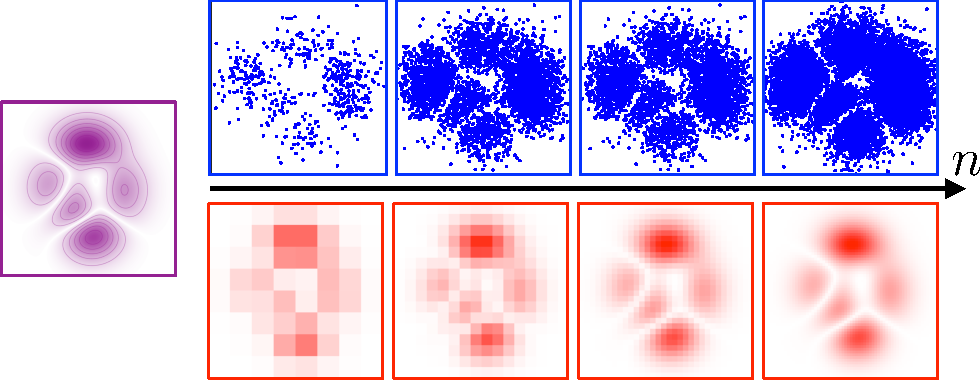
\includegraphics[width=\linewidth]{eulerian-lagrangian/eulerian-lagrangian.pdf}
\caption{\label{fig-eulerian-lagrangian}
Increasing fine discretization of a continuous distribution having a density (violet, left) using a Lagrangian representation $\frac{1}{n}\sum_i \de_{x_i}$ (blue, top) and an Eulerian representation $\sum_i \a_i \de_{x_i}$ with $x_i$ representing cells on a grid of increasing size (red, bottom). The Eulerian perspective starts from a pixelated image down to one with such fine resolution that it almost matches the original density. Weights $\a_i$ are directly proportional to each pixel-cell's intensity.
}
\end{figure}


%%%%%%%%%%%%%%%%%%%%%%%%%%%%%%%%%%%%%
\subsection{Eulerian Discretization}

A first way to discretize the problem is to suppose that both distributions $\be=\sum_{j=1}^m \b_j \de_{y_j}$ and $\al_\th=\sum_{i=1}^n \a(\th)_i \de_{x_i}$ are discrete distributions defined on fixed locations $(x_i)_i$ and $(y_j)_j$. Such locations might stand for cells dividing the entire space of observations in a grid, or a finite subset of points of interest in a continuous space (such as a family of vector embeddings for all words in a given dictionary~\citep{kusner2015word,pmlr-v51-rolet16}). The parameterized measure $\al_\th$ is in that case entirely represented through the weight vector $\a : \th \mapsto \a(\th) \in \Si_n$, which, in practice, might be very sparse if the grid is large. This setting corresponds to the so-called class of Eulerian discretization methods. In its original form, the objective of Problem~\eqref{eq-wloss-generic} is not differentiable. In order to obtain a smooth minimization problem, we use the entropic regularized OT and approximate~\eqref{eq-wloss-generic} using 
\eq{
	\umin{\th \in \Theta} \Ee_E(\th) \eqdef \MKD_\C^\epsilon(\a(\th),\b)
	\qwhereq
	\C_{i,j} \eqdef c(x_i,y_j).
}
We recall that Proposition~\ref{prop-convexity-dual} shows that the entropic loss function is differentiable and convex with respect to the input histograms, with gradient.

%%%%%%%%%%
\begin{proposition}[Derivative with respect to histograms]
For $\epsilon>0$, 
$(\a,\b) \mapsto \MKD_\C^\epsilon(\a,\b)$ is convex and differentiable. Its gradient reads
\eql{\label{eq-diff-marginals}
		\nabla \MKD_\C^\epsilon(\a,\b) = (\fD,\gD),
}
where $(\fD,\gD)$ is the unique solution to~\eqref{eq-dual-formulation}, centered such that $\sum_i \fD_i=\sum_j \gD_j=0$. For $\epsilon=0$, this formula defines the elements of the sub-differential of $\MKD_\C^\epsilon$, and the function is differentiable if they are unique. 
\end{proposition}

The zero mean condition on $(\fD,\gD)$ is important when using gradient descent to guarantee conservation of mass.
%
% \todoK{
% \begin{proof}
% 	Use the dual formulation~\eqref{eq-dual-formulation}. \todoK{write me}
% \end{proof}
% }
% %%%%%%%%%%
Using the chain rule, one thus obtains that $\Ee_E$ is smooth and that its gradient is
\eql{\label{eq-diff-loss-eul}
	\nabla \Ee_E(\th) = [ \partial \a(\th) ]^\top( \fD\, ),
}
where $\partial \a(\th) \in \RR^{n \times \text{dim}(\Theta)}$ is the Jacobian (differential) of the map $\a(\th)$, and 
where $\fD \in \RR^n$ is the dual potential vector associated to the dual entropic OT~\eqref{eq-dual-formulation} between $\a(\th)$ and $\b$ for the cost matrix $\C$ (which is fixed in a Eulerian setting, and in particular independent of $\th$). 
%
This result can be used to minimize locally $\Ee_E$ through gradient descent.

%%%%%%%%%%%%%%%%%%%%%%%%%%%%%%%%%%%%%
\subsection{Lagrangian Discretization}

A different approach consists in using instead fixed (typically uniform) weights and approximating an input measure $\alpha$ as an empirical measure $\al_\th = \frac{1}{n}\sum_i \de_{x(\th)_i}$ for a point-cloud parameterization map $x : \th \mapsto x(\th) = (x(\th)_i)_{i=1}^n \in \Xx^n$, where we assume here that $\X$ is Euclidean. Problem~\eqref{eq-wloss-generic} is thus approximated as
\eql{\label{eq-lagr-sinkloss}
	\umin{\th} \Ee_L(\th) \eqdef \MKD_{\C(x(\th))}^\epsilon(\ones_n/n,\b)
	\qwhereq
	\C(x)_{i,j} \eqdef c(x(\theta)_i,y_j).
}
Note that here the cost matrix $\C(x(\th))$ now depends on $\th$ since the support of $\al_\th$ changes with $\theta$.
%
The following proposition shows that the entropic OT loss is a smooth function of the cost matrix and gives the expression of its gradient.

%%%%%%%%%%
\begin{proposition}[Derivative with respect to the cost]
For fixed input histograms $(\a,\b)$, for $\epsilon>0$, the mapping $\C \mapsto \Rr(\C) \eqdef \MKD_\C^\epsilon(\a,\b)$ is concave and smooth, and  
\eql{\label{eq-diff-cost}
	\nabla \Rr(\C) = \P, 
}
where $\P$ is the unique optimal solution of~\eqref{eq-regularized-discr}. 
%
For $\epsilon=0$, this formula defines the set of upper gradients. 
\end{proposition}
%%%%%%%%%%


\todoK{
\begin{proof}
	Use the primal formulation~\eqref{eq-regularized-discr}. \todoK{write me}
	Formula~\eqref{eq-diff-positions} follows using the chain rule. 
\end{proof}
}

Assuming $(\X,\Y)$ are convex subsets of $\RR^\dim$, for discrete measures $(\al,\be)$ of the form~\eqref{eq-pair-discr}, one obtains using the chain rule that $x = (x_i)_{i=1}^n  \in \X^n \mapsto \Ff(x) \eqdef  \MKD_{\C(x)}(\ones_n/n,\b)$ is smooth and that
\eql{\label{eq-diff-positions}
	\nabla \Ff(x) = \pa{ \sum_{j=1}^m \P_{i,j} \nabla_1 \c(x_i,y_j) }_{i=1}^n \in \X^n,
}
where $\nabla_1 \c$ is the gradient with respect to the first variable. 
%
For instance, for $\X=\Y=\RR^d$, for $\c(s,t) = \norm{s-t}^2$ on $\X=\Y=\RR^d$, one has
\eql{\label{eq-diff-positions-eucl}
	\nabla \Ff(x) = 2 \pa{ \a_i x_i - \sum_{j=1}^m \P_{i,j} y_j }_{i=1}^n,
}
where $\a_i=1/n$ here.
%
Note that, up to a constant, this gradient is $\Id-\T$, where $\T$ is the barycentric projection defined in~\eqref{eq-baryproj}.
%
Using the chain rule, one thus obtains that the Lagrangian discretized problem~\eqref{eq-lagr-sinkloss} is smooth and its gradient is
\eql{\label{eq-diff-loss-lagr}
	\nabla \Ee_L(\th) = [ \partial x(\th) ]^\top( \nabla \Ff( x(\th) ) ),
}
where $\partial x(\th) \in \RR^{\text{dim}(\Theta) \times (n\dim)}$ is the Jacobian of the map $x(\th)$ and
where $\nabla \Ff$ is implemented as in~\eqref{eq-diff-positions} or~\eqref{eq-diff-positions-eucl} using for $\P$ the optimal coupling matrix between $\al_\th$ and $\be$.
%
One can thus implement a gradient descent to compute a local minimizer of $\Ee_L$, as used, for instance, in~\citep{CuturiBarycenter}.

%%%%%%%%%%%%%%%%%%%%%%%%%%%%%%%%%%%%%
\subsection{Automatic Differentiation}
\label{rem-auto-diff}

The difficulty when applying formulas~\eqref{eq-diff-loss-eul} and~\eqref{eq-diff-loss-lagr} is that one needs to compute the exact optimal solutions $\fD$ or $\P$ for these formulas to be valid, which can only be achieved with acceptable precision using a very large number of Sinkhorn iterates.
%
In challenging situations in which the size and the quantity of histograms to be compared are large, the computational budget to compute a single Wasserstein distance is usually limited, therefore allowing only for a few Sinkhorn iterations. In that case, and rather than approximating the gradient~\eqref{eq-dual-formulation} using the value obtained at a given iterate, it is usually better to differentiate directly the output of Sinkhorn's algorithm, using reverse mode automatic differentiation. This corresponds to using the ``algorithmic'' Sinkhorn divergences as introduced in~\eqref{eq-algorithmic-loss}, rather than the quantity $\MKD_\C^\varepsilon$ in~\eqref{eq-regularized-discr} which incorporates the entropy of the regularized optimal transport, and differentiating it directly as a composition of simple maps using the inputs, either the histogram in the Eulerian case or the cost matrix in the Lagrangian cases. Using definitions introduced in~\S\ref{sec-regularized-cost}, this is equivalent to differentiating 
$$\itL{\SINKHORND_{\C}}(\a(\theta),\b) \quad\text{ or }\quad \itL{\SINKHORND_{\C(x(\theta))}}(\a,\b)$$
with respect to $\theta$, in, respectively, the Eulerian and the Lagrangian cases for $L$ large enough.

The cost for computing the gradient of functionals involving Sinkhorn divergences is the same as that of computation of the functional itself; see, for instance,~\citep{2016-bonneel-barycoord,2017-Genevay-AutoDiff} for some applications of this approach. We also refer to~\citep{adams2011ranking} for an early work on differentiating Sinkhorn iterations with respect to the cost matrix (as done in the Lagrangian framework), with applications to learning rankings.
%
Further details on automatic differentiation can be found in~\citep{griewank2008evaluating,rall1981automatic,Neidinger10}, in particular on the ``reverse mode,'' which is the fastest way to compute gradients. 
%
In terms of implementation, all recent deep-learning Python frameworks feature state-of-the-art reverse-mode differentiation and support for GPU/TPU computations~\citep{theano2016,abadi2016tensorflow,pytorch}, they should be adopted for any large-scale application of Sinkhorn losses.
%
We strongly encourage the use of such automatic differentiation techniques, since they have the same complexity as computing~\eqref{eq-diff-loss-eul} and~\eqref{eq-diff-loss-lagr}, these formulas being mostly useful to obtain a theoretical understanding of what automatic differentation is computing. The only downside is that reverse mode automatic differentation is memory intensive (the memory grows proportionally with the number of iterations).  There exist, however, subsampling strategies that mitigate this problem~\citep{griewank1992achieving}.





%%%%%%%%%%%%%%%%%%%%%%%%%%%%%%%%%%%%%
\section{Wasserstein Barycenters, Clustering and Dictionary Learning}
\label{sec-bary}

A basic problem in unsupervised learning is to compute the ``mean'' or ``barycenter'' of several data points. A classical way to define such a weighted mean of points $(x_s)_{s=1}^S \in \X^S$ living in a metric space $(\X,d)$ (where $d$ is a distance or more generally a divergence) is by solving a variational problem 
\eql{\label{eq-frechet-means}
	\umin{x \in \X} \sum_{s=1}^S \la_s d(x,x_s)^p 
}
for a given family of weights $(\la_s)_s \in \simplex_S$, where $p$ is often set to $p=2$. 
%
When $\X=\RR^d$ and $d(x,y)=\norm{x-y}_2$, this leads to the usual definition of the linear average $x=\sum_s \la_s x_s$ for $p=2$ and the more evolved median point when $p=1$. One can retrieve various notions of means (\emph{e.g.} harmonic or geometric means over $\X=\RR_+$) using this formalism.
%
This process is often referred to as the ``Fr\'echet''  or ``Karcher'' mean (see~\citet{karcher2014riemannian} for a historical account). For a generic distance $d$, Problem~\eqref{eq-frechet-means} is usually a difficult nonconvex optimization problem. Fortunately, in the case of optimal transport distances, the problem can be formulated as a convex program for which existence can be proved and efficient numerical schemes exist. 


%%%%%%%%%%%%
\paragraph{Fr\'echet means over the Wasserstein space.}

Given input histogram $\{\b_s\}_{s=1}^S$, where $b_s \in \simplex_{n_s}$, and weights $\la \in \simplex_S$, a Wasserstein barycenter is computed by minimizing
\eql{\label{eq-wass-discr}
	\umin{\a \in \simplex_n} \sum_{s=1}^S \la_s \MKD_{\C_s}(\a,\b_s),
}
where the cost matrices $\C_s \in \RR^{n \times n_s}$ need to be specified. 
%
A typical setup is ``Eulerian,'' so that all the barycenters are defined on the same grid, $n_s=n$, $\C_s=\C=\distD^p$ is set to be a distance matrix, to solve
\eq{
	\umin{\a \in \simplex_n} \sum_{s=1}^S \la_s \WassD_p^p(\a,\b_s). 
}

The barycenter problem~\eqref{eq-wass-discr} was introduced in a more general form involving arbitrary measures in~\citet{Carlier_wasserstein_barycenter} following earlier ideas of~\citet{carlierekelandmatching}. That presentation is deferred to Remark~\ref{rem-bary-carlier}. % They proved in particular uniqueness of the barycenter for $c(x,y)=\norm{x-y}^2$ over $\X=\RR^d$, if one of the input measure has a density with respect to the Lebesgue measure (and more generally under the same hypothesis as the one guaranteeing the existence of a Monge map, see Remark~\ref{rem-exist-mongemap}). ---> THIS SHOULD APPEAR IN THE GREY BOX
The barycenter problem for histograms~\eqref{eq-wass-discr} is in fact a linear program, since one can look for the $S$ couplings $(\P_s)_s$ between each input and the barycenter itself, which by construction must be constrained to share the same row marginal,
\eq{
	\umin{\a \in \simplex_n, (\P_s \in \RR^{n \times n_s})_s } \enscond{
		\sum_{s=1}^S \la_s \dotp{\P_s}{\C_s}
	}{
		\foralls s, \P_s^\top \ones_{n_s}=\a, \P_s^\top \ones_{n} = \b_s
	}.
}
Although this problem is an LP, its scale forbids the use of generic solvers for medium-scale problems. One can resort to using first order methods such as subgradient descent on the dual~\citep{Carlier-NumericsBarycenters}.

%%%%%%%%%%%%%%%%%%%%
\begin{rem2}{Barycenter of arbitrary measures}\label{rem-bary-carlier}
	Given a set of input measure $(\be_s)_s$ defined on some space $\X$, the barycenter problem becomes 
	\eql{\label{eq-barycenter-generic}
		\umin{\al \in \Mm_+^1(\X)} \sum_{s=1}^S \la_s \MK_{\c}(\al,\be_s).
	}
	In the case where $\X=\RR^d$ and $c(x,y)=\norm{x-y}^2$,~\citet{Carlier_wasserstein_barycenter} show that if one of the input measures has a density, then this barycenter is unique. 
	%
	Problem~\eqref{eq-barycenter-generic} can be viewed as a generalization of the problem of computing barycenters of points $(x_s)_{s=1}^S \in \X^S$ to arbitrary measures. Indeed, if $\be_s=\de_{x_s}$ is a single Dirac mass, then a solution to~\eqref{eq-barycenter-generic} is $\de_{x^\star}$, where $x^\star$ is a Fr\'echet mean solving~\eqref{eq-frechet-means}.
	%
	Note that for $c(x,y)=\norm{x-y}^2$, the mean of the barycenter $\al^\star$ is necessarily the barycenter of the mean, \ie 
	\eq{
		\int_\Xx x \d\al^\star(x) =  \sum_s \la_s \int_\Xx x \d\al_s(x), 
	}
	and the support of $\al^\star$ is located in the convex hull of the supports of the $(\al_s)_s$.
	%
	The consistency of the approximation of the infinite-dimensional optimization~\eqref{eq-barycenter-generic} when approximating the input distribution using discrete ones (and thus solving~\eqref{eq-wass-discr} in place) is studied in~\citet{Carlier-NumericsBarycenters}.
	%
	Let us also note that it is possible to recast~\eqref{eq-barycenter-generic} as a multimarginal OT problem; see Remark~\ref{eq-multimarg-bary}. 
\end{rem2}
%%%%%%%%%%%%%%%%%%%%

\begin{rem2}{$k$-means as a Wasserstein variational problem}\label{rem-bary-kmeans}
When the family of input measures $(\be_s)_s$ is limited to but one measure $\be$, this measure is supported on a discrete finite subset of $\X=\RR^{\dim}$, and the cost is the squared Euclidean distance, then one can show that the barycenter problem 
	\eql{\label{eq-barycenter-kmeans}
		\umin{\al \in \Mm_{k}^1(\X)} \MK_{\c}(\al,\be),
	}
where $\al$ is constrained to be a discrete measure with a finite support of size up to $k$, is equivalent to the usual $k$-means problem taking $\be$. Indeed, one can easily show that the centroids output by the $k$-means problem correspond to the support of the solution $\al$ and that its weights correspond to the fraction of points in $\be$ assigned to each centroid. One can show that approximating $\MK_{\c}$ using entropic regularization results in smoothed out assignments that appear in soft-clustering variants of $k$-means, such as mixtures of Gaussians~\citep{dessein2017parameter}.
\end{rem2}

%%%%%%%%%%%%%%%%%%%%
\begin{rem2}{Distribution of distributions and consistency}
	It is possible to generalize~\eqref{eq-barycenter-generic} to a possibly infinite collection of measures. This problem is described by considering a probability distribution $M$ over the space $\Mm_+^1(\X)$ of probability distributions, \ie $M \in \Mm_+^1(\Mm_+^1(\X))$. A barycenter is then a solution of 
	\eql{\label{eq-bary-infinite} 
		\umin{\al \in \Mm_+^1(\X)} \EE_M( \MK_{\c}(\al,\be) ) = \int_{\Mm_+^1(\X)} \MK_{\c}(\al,\be) \d M(\be), 
	}
	where $\be$ is a random measure distributed according to $M$. Drawing uniformly at random a finite number $S$ of input measures $(\be_s)_{s=1}^S$ according to $M$, one can then define $\hat \be_S$ as being a solution of~\eqref{eq-barycenter-generic} for uniform weights $\la_s=1/S$ (note that here $\hat \be_S$ is itself a random measure). 
	%
	Problem~\eqref{eq-barycenter-generic} corresponds to the special case of a ``discrete'' measure $M=\sum_s \la_s \de_{\be_s}$.
	%
	The convergence (in expectation or with high probability) of $\MK_{\c}(\hat\be_S,\al)$ to zero (where $\al$ is the unique solution to~\eqref{eq-bary-infinite}) corresponds to the consistency of the barycenters, and is proved in~\citep{BigotBarycenter,leGouic2016existence,bigot2012characterization}.
	%
	This can be interpreted as a law of large numbers over the Wasserstein space. The extension of this result to a central limit theorem is an important problem; see~\citep{panaretos2016amplitude} and~\citep{agueh2017vers} for recent formulations of that problem and solutions in particular cases (1-D distributions and Gaussian measures).
\end{rem2}
%%%%%%%%%%%%%%%%%%%%


%%%%%%%%%%%%%%%%%%%%
\begin{rem2}{Fixed-point map}
When dealing with the Euclidean space $\X=\RR^\dim$ with ground cost $\c(x,y)=\norm{x-y}^2$, it is possible to study the barycenter problem using transportation maps. Indeed, if $\al$ has a density, according to Remark~\ref{rem-exist-mongemap}, one can define optimal transportation maps $\T_s$ between $\al$ and $\al_s$, in particular such that $\T_{s,\sharp}\al = \al_s$. The average map 
\eq{
	\T^{(\al)} \eqdef \sum_{s=1}^S \la_s \T_s
} 
(the notation above makes explicit the dependence of this map on $\al$) is itself an optimal map between $\al$ and $\T^{(\al)}_\sharp \al$ (a positive combination of optimal maps is equal by Brenier's theorem, Remark~\ref{rem-exist-mongemap}, to the sum of gradients of convex functions, equal to the gradient of a sum of convex functions, and therefore optimal by Brenier's theorem again). 
As shown in~\citep{Carlier_wasserstein_barycenter}, first order optimality conditions of the barycenter problem~\eqref{eq-bary-infinite} actually read $\T^{(\al^\star)}=\Identity_{\RR^\dim}$ (the identity map) at the optimal measure $\al^\star$ (the barycenter), and it is shown in~\citep{alvarez2016fixed} that the barycenter $\al^\star$ is the unique (under regularity conditions clarified in~\citep[Theo. 2]{zemel2017fr}) to the fixed-point equation 
\eql{\label{eq-fixed-point-bary}
	G(\al) = \al
	\qwhereq 
	G(\al) \eqdef \T^{(\al)}_\sharp \al,
}  
Under mild conditions on the input measures,~\citet{alvarez2016fixed} and~\citet{zemel2017fr} have shown that $\al \mapsto G(\al)$ strictly decreases the objective function of~\eqref{eq-bary-infinite} if $\al$ is not the barycenter and that the fixed-point iterations $\itt{\al} \eqdef G( \it{\al} )$ converge to the barycenter $\al^\star$. 
%
This fixed point algorithm can be used in cases where the optimal transportation maps are known in closed form (\emph{e.g.} for Gaussians). Adapting this algorithm for empirical measures of the same size results in computing optimal assignments in place of Monge maps. For more general discrete measures of arbitrary size the scheme can also be adapted~\citep{CuturiBarycenter} using barycentric projections~\eqref{eq-baryproj}.
\end{rem2}
%%%%%%%%%%%%%%%%%%%%



%%%%%%%%%%%%
\paragraph{Special cases.}

In general, solving~\eqref{eq-wass-discr} or~\eqref{eq-barycenter-generic} is not straightforward, but there exist some special cases for which solutions are explicit or simple. 


%%%%%%%%%%%%%%%%%%%%
\begin{rem1}{Barycenter of Gaussians}
	It is shown in~\citep{Carlier_wasserstein_barycenter} that the barycenter of Gaussians distributions $\al_s = \Nn(\mean_s,\cov_s)$, for the squared Euclidean cost $c(x,y)=\norm{x-y}^2$, is itself a Gaussian $\Nn(\mean^\star,\cov^\star)$.
	%	
	Making use of~\eqref{eq-dist-gauss}, one sees that the barycenter mean is the mean of the inputs
	\eq{
		\mean^\star = \sum_s \la_s \mean_s
	}
	while the covariance minimizes 
	\eq{
		\umin{ \cov } \sum_s \la_s \Bb(\cov,\cov_s)^2,
	}
	where $\Bb$ is the Bure metric~\eqref{eq-bure-defn}. As studied in~\citep{Carlier_wasserstein_barycenter}, the first order optimality condition of this convex problem shows that $\cov^\star$ is the unique positive definite fixed point of the map
	\eq{
		\cov^\star = \Psi(\cov^\star)
		\qwhereq
		\Psi(\cov) \eqdef \sum_s \la_s ( \cov^{\frac{1}{2}} \cov_s \cov^{\frac{1}{2}}  )^{\frac{1}{2}},
	}
	where $\cov^{\frac{1}{2}}$ is the square root of positive semidefinite matrices. 
	%
	This result was known from~\citep{KnottSmith,RuschendorfUckelmann} and is proved in~\citep{Carlier_wasserstein_barycenter}. 
	%
	While $\Psi$ is not strictly contracting, iterating this fixed-point map, \ie defining $\itt{\cov} \eqdef \Psi( \it{\cov} )$ converges in practice to the solution $\cov^\star$.
	% has been shown by~\citet{SuvritSra} to converge to the solution $\cov^\star$.
		% 
	This method has been applied to texture synthesis in~\citep{2014-xia-siims}. \citet{alvarez2016fixed} have also proposed to use an alternative map 
	\eq{
		\bar\Psi(\cov) \eqdef 
		\cov^{-\frac{1}{2}} 
		\Big( \sum_s \la_s ( \cov^{\frac{1}{2}} \cov_s \cov^{\frac{1}{2}}  )^{\frac{1}{2}} \Big)^2 
		\cov^{-\frac{1}{2}}
	}
	for which the iterations $\itt{\cov} \eqdef \bar\Psi( \it{\cov} )$ converge.
	%
	This is because the fixed-point map $G$ defined in~\eqref{eq-fixed-point-bary} preserves Gaussian distributions, and in fact, 
	\eq{
		G( \Nn(\mean,\cov) ) = \Nn(\mean^\star,\bar\Psi(\cov)). 		
	}
	%
	Figure~\ref{fig-bary-gaussian} shows two examples of computations of barycenters between four 2-D Gaussians.
\end{rem1}
%%%%%%%%%%%%%%%%%%%%



\begin{figure}[h!]
\centering
\begin{tabular}{@{}c@{\hspace{20mm}}c@{}}
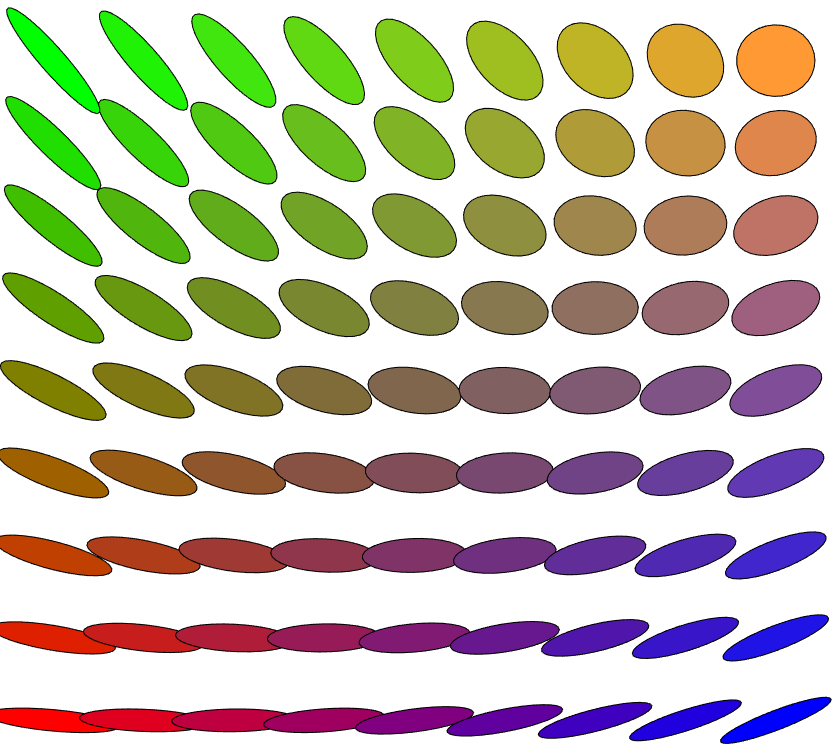
\includegraphics[width=.3\linewidth]{barycenters-gaussians/tensor-interp-70} &
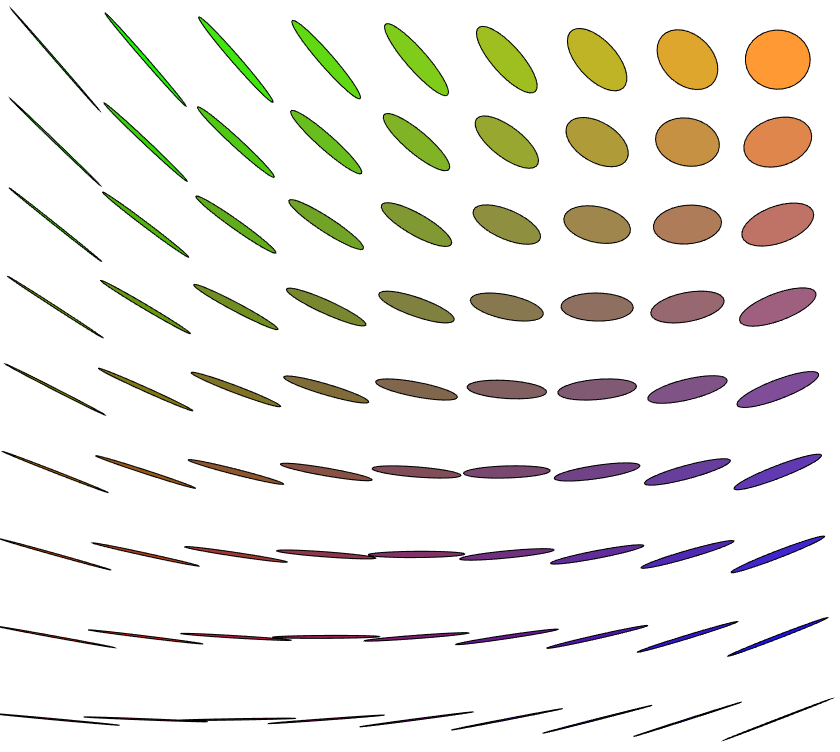
\includegraphics[width=.3\linewidth]{barycenters-gaussians/tensor-interp-98} 
\end{tabular}
\caption{\label{fig-bary-gaussian}
Barycenters between four Gaussian distributions in 2-D. Each Gaussian is displayed using an ellipse aligned with the principal axes of the covariance, and with elongations proportional to the corresponding eigenvalues. 
}
\end{figure}


%%%%%%%%%%%%%%%%%%%%
\begin{rem1}{1-D cases}\label{rem-bary-1d}
	For 1-D distributions, the $\Wass_p$ barycenter can be computed almost in closed form using the fact that the transport is the monotone rearrangement, as detailed in Remark~\ref{rem-1d-ot-generic}. 
	% 
	The simplest case is for empirical measures with $n$ points, \ie $\be_s = \frac{1}{n}\sum_{i=1}^n \de_{y_{s,i}}$, where the points are assumed to be sorted $y_{s,1} \leq y_{s,2} \leq \ldots$. Using~\eqref{eq-1d-empirical} the barycenter $\al_\la$ is also an empirical measure on $n$ points
	\eq{
		\al_\la = \frac{1}{n}\sum_{i=1}^n \de_{x_{\la,i}}
		\qwhereq
		x_{\la,i} = A_\la(x_{s,i})_s, 
	}
	where $A_\la$ is the barycentric map
	\eq{
	 	A_\la(x_s)_s \eqdef \uargmin{x \in \RR} \sum_{s=1}^S \la_s |x-x_{s}|^p.
	}
	For instance, for $p=2$, one has $x_{\la,i} = \sum_{s=1}^S \la_s x_{s,i}$. 
	%
	In the general case, one needs to use the cumulative functions as defined in~\eqref{eq-cumul-defn}, and using~\eqref{eq-wass-cumul}, one has
	\eq{
		\foralls r \in [0,1], \quad
		\cumul{\al_\la}^{-1}(r) = A_\la( \cumul{\al_s}^{-1}(r) )_{s=1}^S, 
	}
	which can be used, for instance, to compute barycenters between discrete measures supported on less than $n$ points in $O(n\log(n))$ operations, using a simple sorting procedure.
\end{rem1}
%%%%%%%%%%%%%%%%%%%%



%%%%%%%%%%%%%%%%%%%%
\begin{rem1}{Simple cases}
	Denoting by $\T_{r,u} : x \mapsto rx+u$ a scaling and translation, and assuming that $\al_{s} = T_{r_s,u_s,\sharp} \al_0$ is obtained by scaling and translating an initial template measure, then a barycenter $\al_\la$ is also obtained using scaling and translation \todoK{to check}
	\eq{
		\al_\la = T_{r^\star,u^\star,\sharp} \al_0
		\qwhereq
		\choice{
			r^\star = (\sum_s \la_s/r_s)^{-1},  \\
			u^\star = \sum_s \la_s u_s.
		}
	}	
\end{rem1}
%%%%%%%%%%%%%%%%%%%%


%%%%%%%%%%%%%%%%%%%%
\begin{rem1}{Case $S=2$}
	In the case where $\X=\RR^d$ and $c(x,y)=\norm{x-y}^2$ (this can be extended more generally to geodesic spaces), the barycenter between $S=2$ measures $(\al_0,\al_1)$ is the McCann interpolant as already introduced in~\eqref{eq-mc-cann-interp}. Denoting $\T_\sharp \al_0=\al_1$ the Monge map, one has that the barycenter $\al_\la$ reads $\al_\la = (\la_1 \Id + \la_2 \T)_{\sharp} \al_0$.
	%
	Formula~\eqref{eq-mccann-discrete} explains how to perform the computation in the discrete case.
\end{rem1}
%%%%%%%%%%%%%%%%%%%%



%%%%%%%%%%%%
\paragraph{Entropic approximation of barycenters.}

One can use entropic smoothing and approximate the solution of~\eqref{eq-wass-discr} using 
\eql{\label{eq-entropic-bary}
	\umin{\a \in \simplex_n} \sum_{s=1}^S \la_s \MKD_{\C_s}^\epsilon(\a,\b_s)
}
for some $\epsilon>0$. 
%
This is a smooth convex minimization problem, which can be tackled using gradient descent~\citep{CuturiBarycenter,GramfortPC15}. An alternative is to use descent methods (typically quasi-Newton) on the semi-dual~\citep{2016-Cuturi-siims}, which is useful to integrate additional regularizations on the barycenter, to impose, for instance, some smoothness w.r.t a given norm.
%
A simpler yet very effective approach, as remarked by~\citet{2015-benamou-cisc} is to rewrite~\eqref{eq-entropic-bary} as a (weighted) KL projection problem
\eql{\label{eq-bary-entropy-couplings}
	\umin{ (\P_s)_s } \enscond{ \sum_{s} \la_s \epsilon \KLD( \P_s|\K_s ) }{
		\foralls s, \transp{\P_s}\ones_m = \b_s, \:
		\P_1\ones_1 =  \cdots = \P_S\ones_S,
	}
}
where we denoted $\K_s \eqdef e^{-\C_s/\epsilon}$. Here, the barycenter $\a$ is implicitly encoded in the row marginals of all the couplings $\P_s \in \RR^{n \times n_s}$ as $\a = \P_1\ones_1 =  \cdots = \P_S\ones_S$.
%
As detailed by~\citet{2015-benamou-cisc}, one can generalize Sinkhorn to this problem, which also corresponds to iterative projections. This can also be seen as a special case of the generalized Sinkhorn detailed in~\S\ref{sec-generalized}.
%
The optimal couplings $(\P_s)_s$ solving~\eqref{eq-bary-entropy-couplings} are computed in scaling form as 
\eql{\label{eq-bary-opt}
	\P_s=\diag(\uD_s)\K\diag(\vD_s), 
}
and the scalings are sequentially updated as
\begin{align}\label{eq-sinkhorn-bary}
	\foralls s \in \range{1,S}, \quad \itt{\vD}_s &\eqdef \frac{\b_s}{\transp{\K}_s \it{\uD}_s}, \\
	\foralls s \in \range{1,S}, \quad  \itt{\uD}_s &\eqdef \frac{\itt{\a}}{\K_s \itt{\vD}_s}, \label{eq-sinkhorn-bary-2}\\
		\qwhereq
		\itt{\a} &\eqdef \prod_s (  \K_s \itt{\vD}_s )^{\la_s}. \label{eq-sinkhorn-bary-3}
\end{align}
An alternative way to derive these iterations is to perform alternate minimization on the variables of a dual problem, which is detailed in the following proposition.

\begin{prop}
	The optimal $(\uD_s,\vD_s)$ appearing in~\eqref{eq-bary-opt} can be written as $(\uD_s,\vD_s) = ( e^{\fD_s/\epsilon},e^{\gD_s/\epsilon} )$, where $( \fD_s,\gD_s )_s$ are the solutions of the following program (whose value matches the one of \eqref{eq-entropic-bary}):
	\eql{\label{eq-dual-bary-entropy}
		\umax{ ( \fD_s,\gD_s )_s } \enscond{
		\sum_s \la_s \pa{
			\dotp{\gD_s}{\b_s} - \epsilon \dotp{\K_s e^{\gD_s/\epsilon}}{e^{\fD_s/\epsilon}}
		}
		}{
			\sum_s \la_s \fD_s = 0
		}.
	}
\end{prop}

\begin{proof}	Introducing Lagrange multipliers in~\eqref{eq-bary-entropy-couplings} leads to
	\begin{align*}
		\umin{ (\P_s)_s, \a } 
		\umax{ ( \fD_s,\gD_s )_s }
		\sum_{s} \la_s \Big(
			\epsilon \KLD( \P_s|\K_s )
			+ 
			\dotp{\a - \P_s\ones_m}{ \fD_s } \\
		\qquad\qquad	+			
			\dotp{\b_s - \transp{\P_s}\ones_m}{ \gD_s }
		\Big).
	\end{align*}
	Strong duality holds, so that one can exchange the min and the max, to obtain
		\begin{align*}
		&\umax{ ( \fD_s,\gD_s )_s }
			\sum_s \la_s \pa{
				 \dotp{\gD_s}{\b_s}
		+ 
		\umin{\P_s} \epsilon \KLD( \P_s|\K_s ) - \dotp{\P_s}{\fD_s \oplus \gD_s }
		} \\
	&\qquad\qquad	+ \umin{\a}
			\dotp{ \sum_{s} \la_s \fD_s }{\a}.
	\end{align*}
	The explicit minimization on $\a$ gives the constraint $\sum_{s} \la_s \fD_s=0$ together with 
	\begin{align*}
		\umax{ ( \fD_s,\gD_s )_s }
			\sum_s \la_s 
				 \dotp{\gD_s}{\b_s}
		-
		\epsilon \KLD^*\pa{ \frac{\fD_s \oplus \gD_s}{\epsilon}|\K_s },
	\end{align*}
	where $\KLD^*(\cdot|\K_s)$ is the Legendre transform~\eqref{eq-legendre} of the function $\KLD^*(\cdot|\K_s)$.
	%
	This Legendre transform reads
	\eql{\label{eq-legendre-kl}
		\KLD^*(\VectMode{U}|\K) = \sum_{i,j} \K_{i,j} (e^{\VectMode{U}_{i,j}}-1), 
	}
	which shows the desired formula. 
	%
	To show~\eqref{eq-legendre-kl}, since this function is separable, one needs to compute
	\eq{
		\foralls (u,k) \in \RR_+^2, \quad
		\KLD^*(u|k) \eqdef \umax{r} ur -   \pa{ r \log(r/k) - r + k  }
	}
	whose optimality condition reads $u=\log(r/k)$, \ie $r = k e^{u}$, hence the result.
\end{proof}

Minimizing~\eqref{eq-dual-bary-entropy} with respect to each $\gD_s$, while keeping all the other variables fixed, is obtained in closed form by~\eqref{eq-sinkhorn-bary}. 
%
Minimizing~\eqref{eq-dual-bary-entropy} with respect to all the $(\fD_s)_s$ requires us to solve for $\a$ using~\eqref{eq-sinkhorn-bary-3} and leads to the expression~\eqref{eq-sinkhorn-bary-2}.



Figures~\ref{fig-barycenters-images} and~\ref{fig-barycenters-shapes} show applications to 2-D and 3-D shapes interpolation. Figure~\ref{fig-barycenters-surfaces} shows a computation of barycenters on a surface, where the ground cost is the square of the geodesic distance. For this figure, the computations are performed using the geodesic in heat approximation detailed in Remark~\ref{rem-geod-heat}. We refer to~\citep{2015-solomon-siggraph} for more details and other applications to computer graphics and imaging sciences.

%
\newcommand{\FigBaryImA}[2]{\includegraphics[width=.088\linewidth]{barycenters-2d/annulus-cross-heart-2disk/shape-#1-#2}}
\newcommand{\FigBaryImLineA}[1]{\FigBaryImA{#1}{1} & \FigBaryImA{#1}{2} & \FigBaryImA{#1}{3} & \FigBaryImA{#1}{4} & \FigBaryImA{#1}{5}}
\newcommand{\FigBaryImB}[2]{\includegraphics[width=.088\linewidth]{barycenters-2d/cat-star8-thinspiral-trefle/shape-#1-#2}}
\newcommand{\FigBaryImLineB}[1]{\FigBaryImB{#1}{1} & \FigBaryImB{#1}{2} & \FigBaryImB{#1}{3} & \FigBaryImB{#1}{4} & \FigBaryImB{#1}{5}}


\begin{figure}[h!]
\centering
\fbox{
\begin{tabular}{@{}c@{}c@{}c@{}c@{}c@{}}
\FigBaryImLineA{1} \\
\FigBaryImLineA{2} \\
\FigBaryImLineA{3} \\
\FigBaryImLineA{4} \\
\FigBaryImLineA{5}
\end{tabular}
}
\fbox{
\begin{tabular}{@{}c@{}c@{}c@{}c@{}c@{}}
\FigBaryImLineB{1} \\
\FigBaryImLineB{2} \\
\FigBaryImLineB{3} \\
\FigBaryImLineB{4} \\
\FigBaryImLineB{5}
\end{tabular}
}
\caption{\label{fig-barycenters-images}
Barycenters between four input 2-D shapes using entropic regularization~\eqref{eq-entropic-bary}. To display a binary shape, the displayed images shows a thresholded density. 
%
The weights $(\la_s)_s$ are bilinear with respect to the four corners of the square.  
}
\end{figure}



% trim=left bottom right height
\newcommand{\FigBaryShapeA}[2]{\includegraphics[width=.09\linewidth,trim=130 78 110 60,clip]{barycenters-shapes/duck-spiky-moomoo_s0-double-torus/barycenter-#1-#2}}
\newcommand{\FigBaryShapeLineA}[1]{\FigBaryShapeA{#1}{0} & \FigBaryShapeA{#1}{1} & \FigBaryShapeA{#1}{2} & \FigBaryShapeA{#1}{3} & \FigBaryShapeA{#1}{4}}
%
\newcommand{\FigBaryShapeB}[2]{\includegraphics[width=.087\linewidth,trim=160 65 150 55,clip]{barycenters-shapes/mushroom-torus-hand1-trim-star/barycenter-#1-#2}}
\newcommand{\FigBaryShapeLineB}[1]{\FigBaryShapeB{#1}{0} & \FigBaryShapeB{#1}{1} & \FigBaryShapeB{#1}{2} & \FigBaryShapeB{#1}{3} & \FigBaryShapeB{#1}{4}}

\begin{figure}[h!]
\centering
%%% VOLUMETRIC SHAPES %%%
\fbox{
\begin{tabular}{@{}c@{}c@{}c@{}c@{}c@{}}
\FigBaryShapeLineA{0} \\
\FigBaryShapeLineA{1} \\
\FigBaryShapeLineA{2} \\
\FigBaryShapeLineA{3} \\
\FigBaryShapeLineA{4}
\end{tabular}
}
\fbox{
\begin{tabular}{@{}c@{}c@{}c@{}c@{}c@{}}
\FigBaryShapeLineB{0} \\
\FigBaryShapeLineB{1} \\
\FigBaryShapeLineB{2} \\
\FigBaryShapeLineB{3} \\
\FigBaryShapeLineB{4}
\end{tabular}
}
\caption{\label{fig-barycenters-shapes}
Barycenters between four input 3-D shapes using entropic regularization~\eqref{eq-entropic-bary}. The weights $(\la_s)_s$ are bilinear with respect to the four corners of the square.  
%
Shapes are represented as measures that are uniform within the boundaries of the shape and null outside.
}
\end{figure}
The efficient computation of Wasserstein barycenters remains at this time an active research topic~\citep{NIPS2017_6858,NIPS2018_8274}. Beyond their methodological interest, Wasserstein barycenters have found many applications outside the field of shape analysis. They have been used for image processing~\citep{rabin-ssvm-11}, in particular color modification~\citep{2015-solomon-siggraph} (see Figure~\ref{fig-colors}); Bayesian computations~\citep{srivastava2015scalable,srivastava2015wasp} to summarize measures; and nonlinear dimensionality reduction, to express an input measure as a Wasserstein barycenter of other known measures~\citep{2016-bonneel-barycoord}. All of these problems result in involved nonconvex objective functions which can be accurately optimized using automatic differentiation (see Remark~\ref{rem-auto-diff}). 
%
Problems closely related to the computation of barycenters include the computation of principal components analyses over the Wasserstein space (see, for instance,~\citep{SeguyCuturi,bigot2017geodesic}) and the statistical estimation of template models~\citep{boissard2015distribution}. The ability to compute barycenters enables more advanced clustering methods such as the $k$-means on the space of probability measures~\citep{del2016robust,ho2017multilevel}.




\begin{figure}[h!]
\centering
\begin{tabular}{@{}c@{}c@{}c@{}c@{}c@{}}
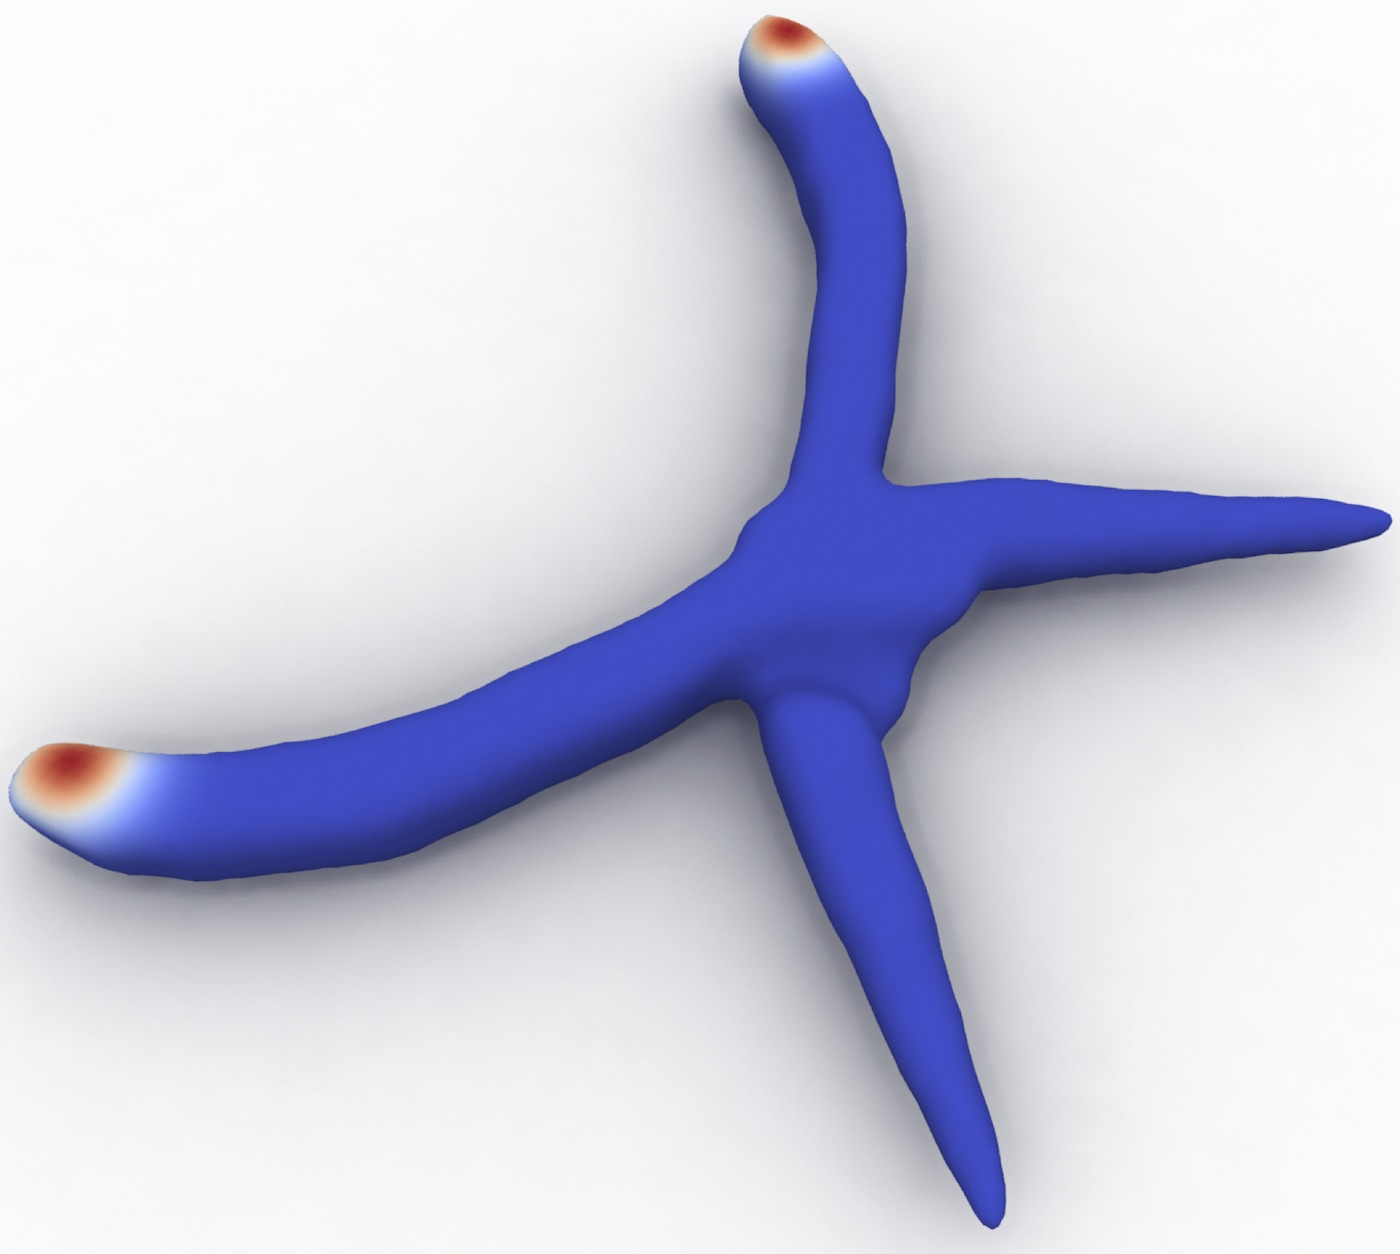
\includegraphics[width=.195\linewidth]{barycenters-surfaces/scisor-1}&
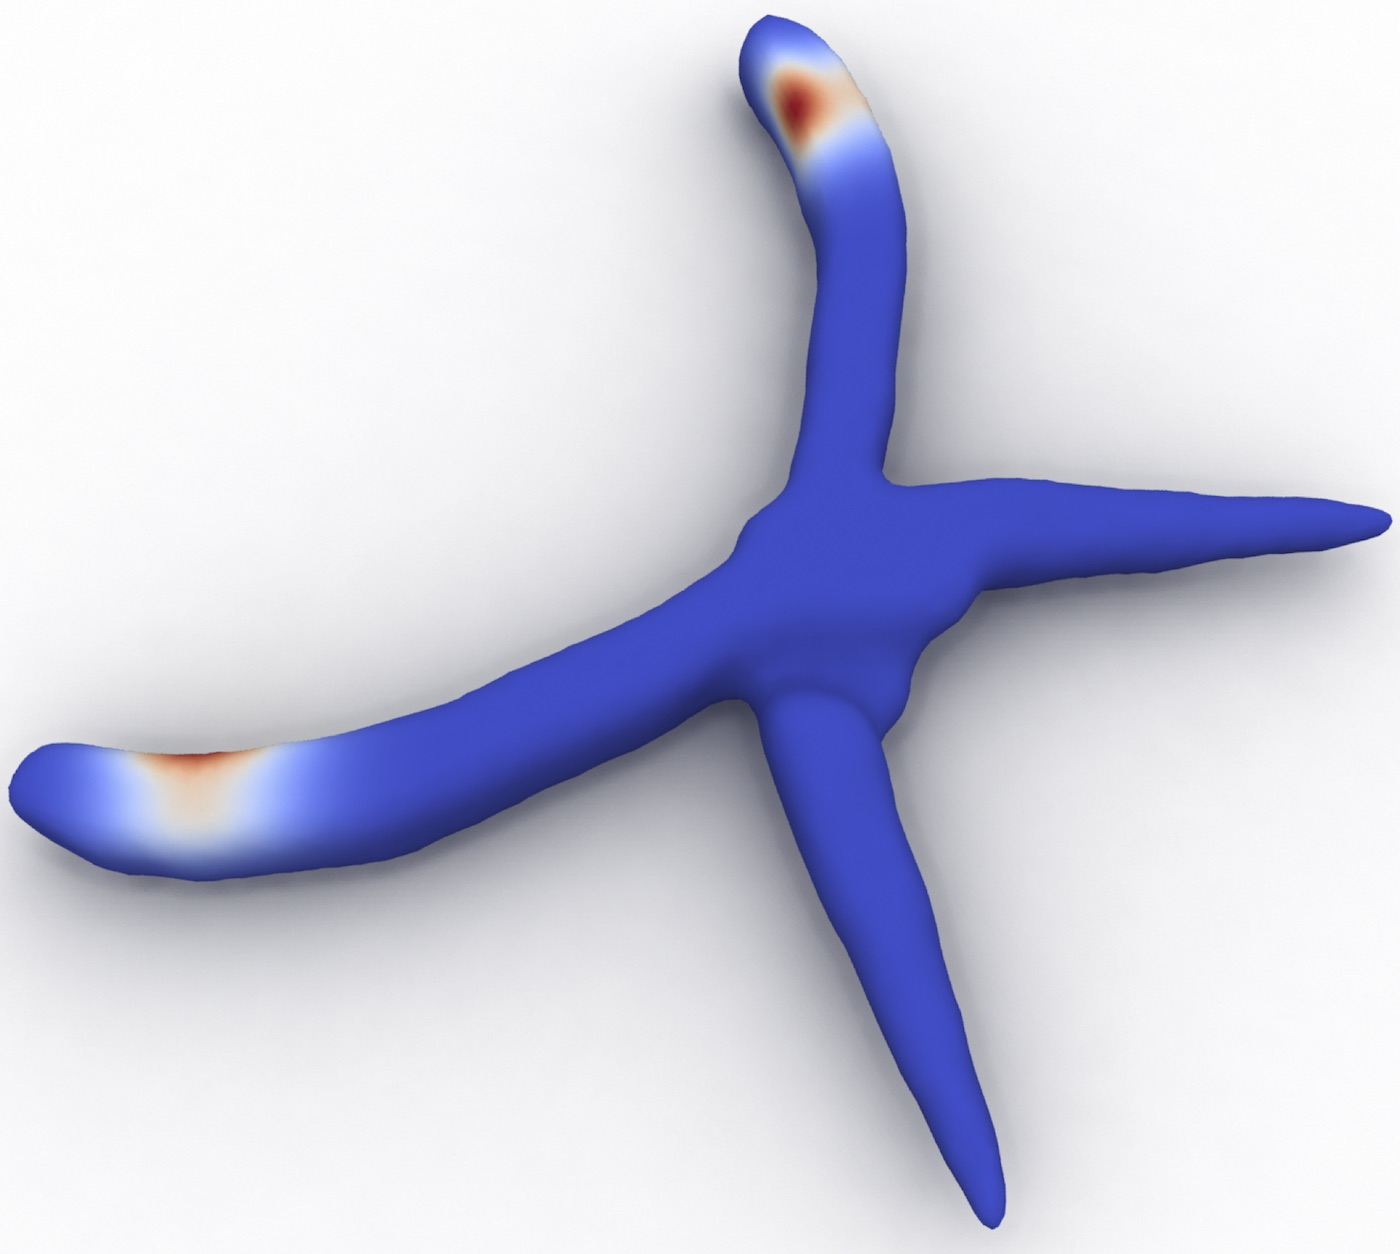
\includegraphics[width=.195\linewidth]{barycenters-surfaces/scisor-2}&
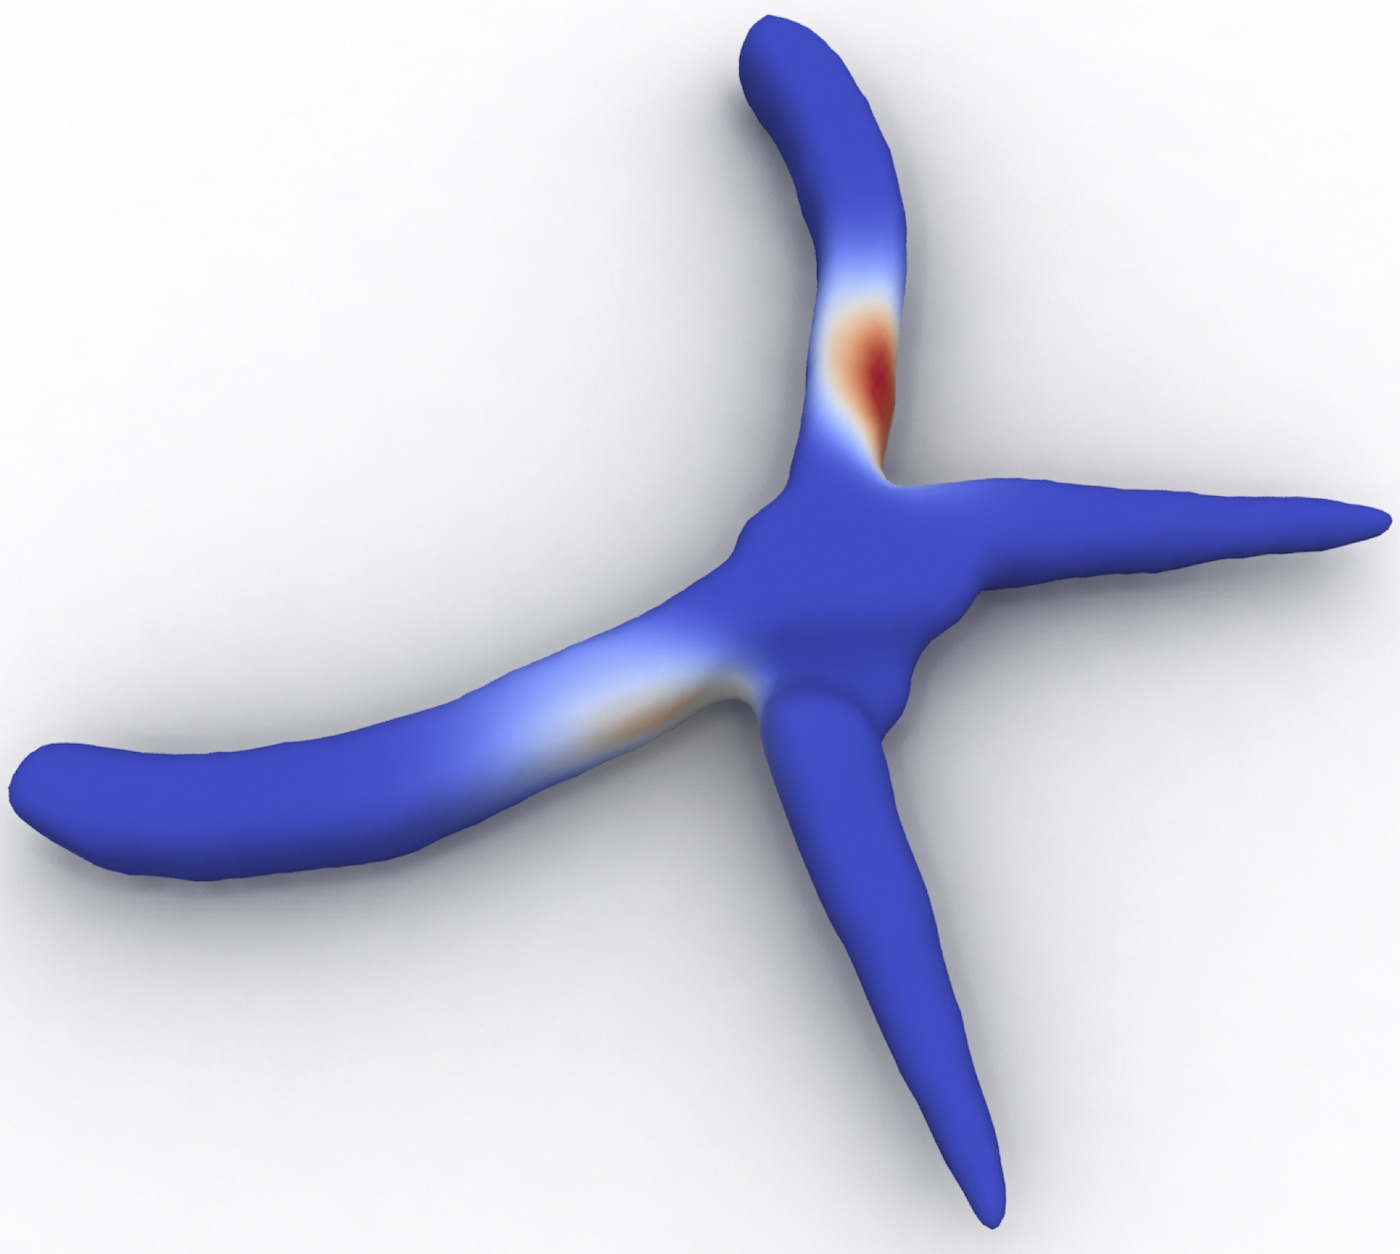
\includegraphics[width=.195\linewidth]{barycenters-surfaces/scisor-3}&
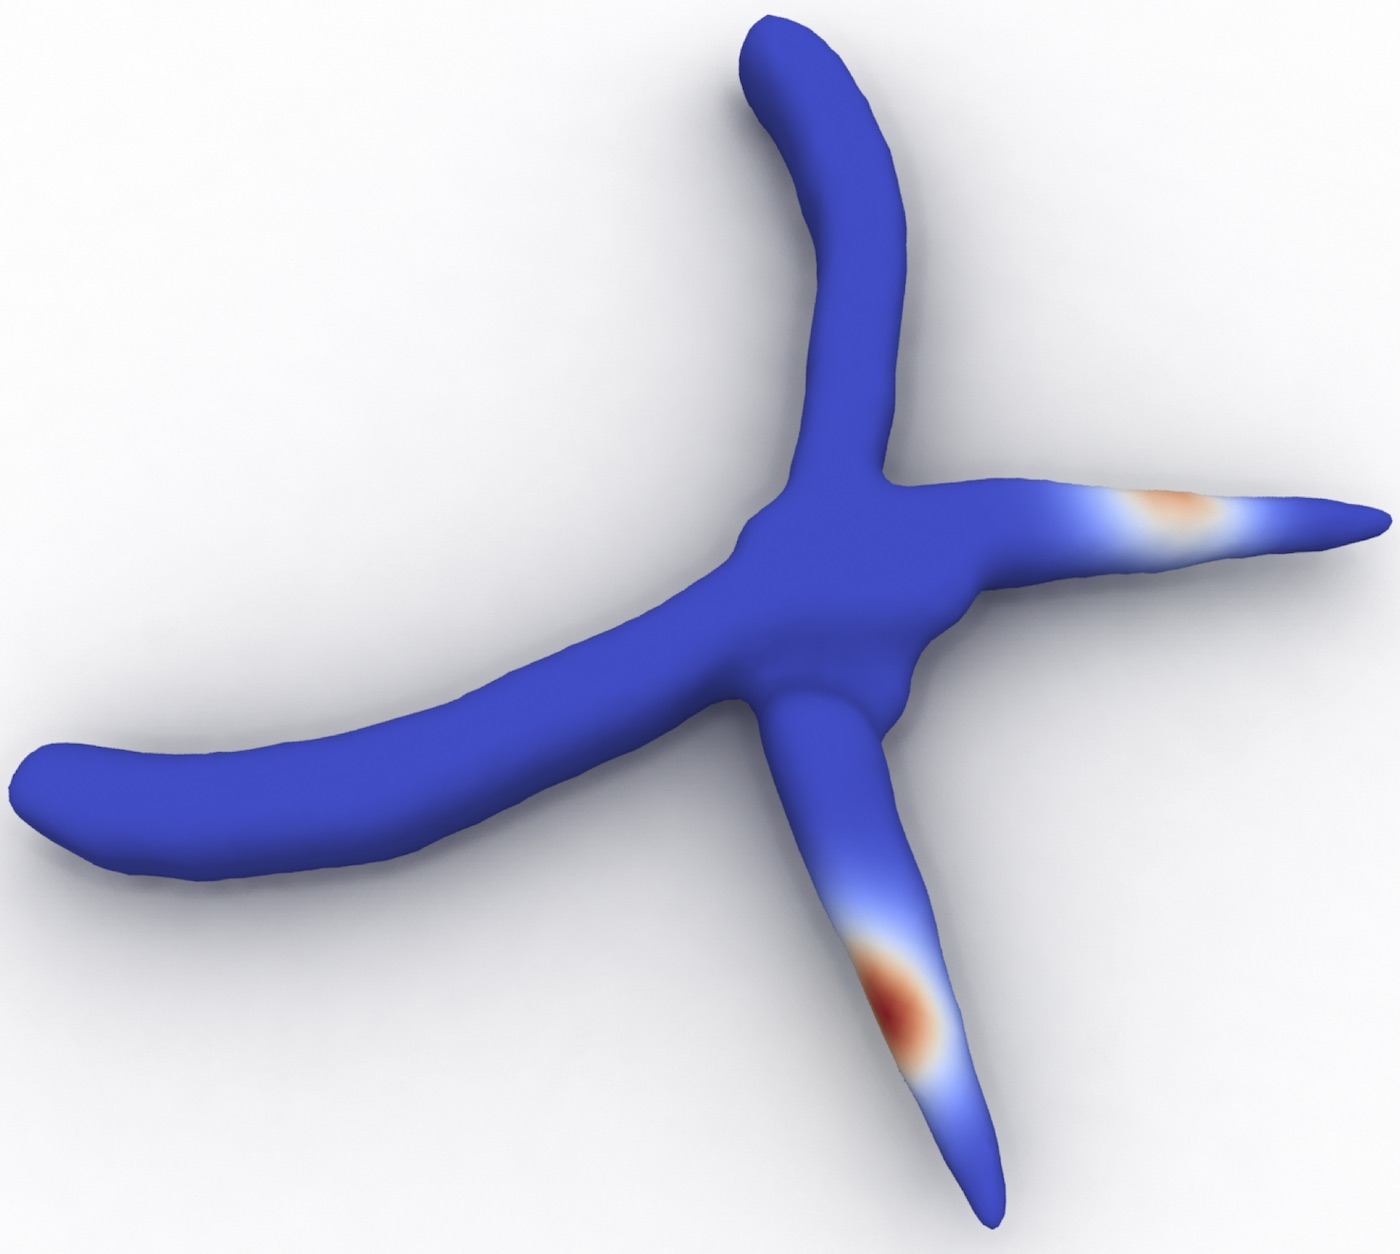
\includegraphics[width=.195\linewidth]{barycenters-surfaces/scisor-4}&
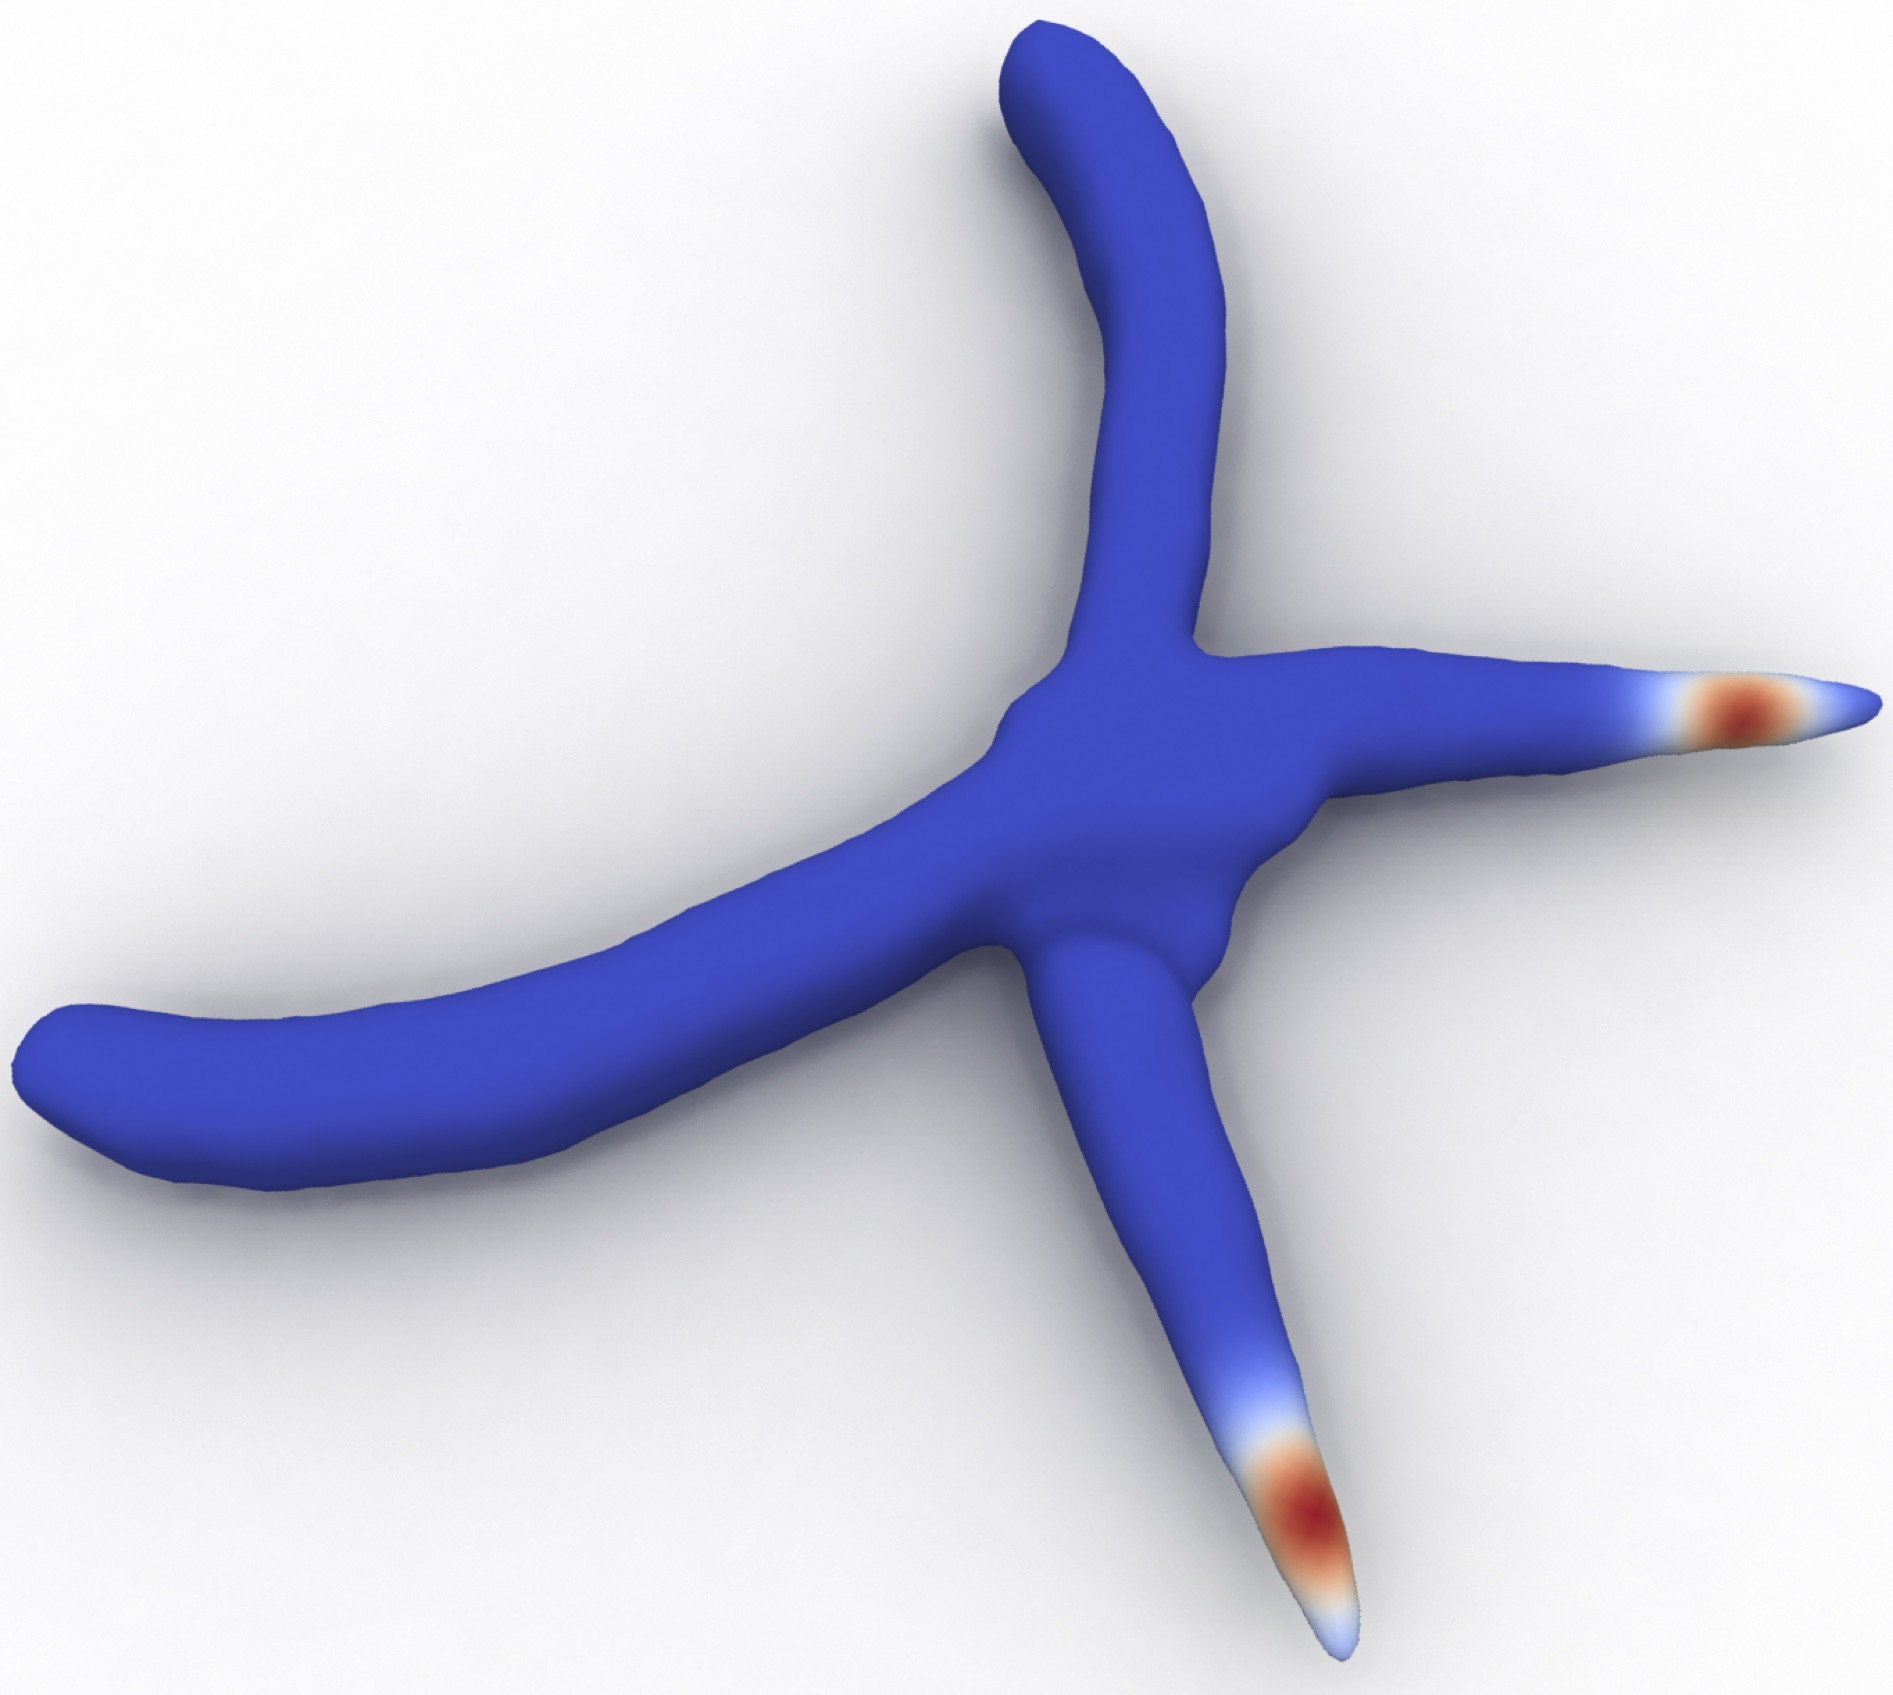
\includegraphics[width=.195\linewidth]{barycenters-surfaces/scisor-5}
\end{tabular}
\caption{\label{fig-barycenters-surfaces}
Barycenters interpolation between two input measures on surfaces, computed using the geodesic in heat fast kernel approximation (see Remark~\ref{rem-geod-heat}). Extracted from~\citep{2015-solomon-siggraph}.
}
\end{figure}



\begin{figure}[h!]
\centering
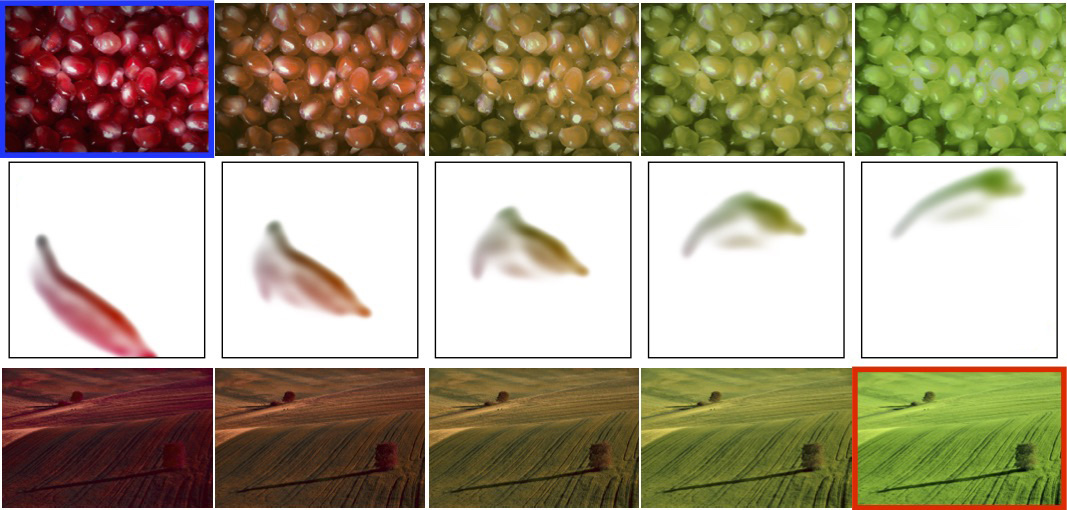
\includegraphics[width=1\linewidth]{colors/colors-bary}
\caption{\label{fig-colors}
Interpolation between the two 3-D color empirical histograms of two input images (here only the 2-D chromatic projection is visualized for simplicity). The modified histogram is then applied to the input images using barycentric projection as detailed in Remark~\ref{rem-barycenric-proj}. Extracted from~\citep{2015-solomon-siggraph}.
}
\end{figure}



%%%%%%%%%%%%%%%%%%%%
\begin{rem1}{Wasserstein propagation}
	As studied in~\citet{Solomon-ICML}, it is possible to generalize the barycenter problem~\eqref{eq-wass-discr}, where one looks for distributions $(\b_u)_{u \in U}$ at some given set $U$ of nodes in a graph $\Gg$ given a set of fixed input distributions $(\b_v)_{v \in V}$ on the complementary set $V$ of the nodes. The unknown are determined by minimizing the overall transportation distance between all pairs of nodes $(r,s) \in \Gg$ forming edges in the graph
	\eql{\label{eq-w-propag}
		\umin{(\b_u  \in \simplex_{n_u})_{u \in U}} 
			\sum_{(r,s) \in \Gg}  \MKD_{\C_{r,s}}(\b_r,\b_s),
	}
	where the cost matrices $\C_{r,s} \in \RR^{n_r \times n_s}$ need to be specified by the user.
	%
	The barycenter problem~\eqref{eq-wass-discr} is a special case of this problem where the considered graph $\Gg$ is ``star shaped,'' where $U$ is a single vertex connected to all the other vertices $V$ (the weight $\la_s$ associated to $\b_s$ can be absorbed in the cost matrix). 
	%
	Introducing explicitly a coupling $\P_{r,s} \in \CouplingsD( \b_r,\b_s )$ for each edge $(r,s) \in \Gg$, and using entropy regularization, one can rewrite this problem similarly as in~\eqref{eq-bary-entropy-couplings}, and one extends Sinkhorn iterations~\eqref{eq-sinkhorn-bary} to this problem (this can also be derived by recasting this problem in the form of the generalized Sinkhorn algorithm detailed in~\S\ref{sec-generalized}). 
	% 
	\todoK{show a graphical illustration}
	%
	This discrete variational problem~\eqref{eq-w-propag} on a graph can be generalized to define a Dirichlet energy when replacing the graph by a continuous domain~\citep{solomon2013dirichlet}. This in turn leads to the definition of measure-valued harmonic functions which finds application in image and surface  processing. We refer also to~\citet{Lavenant2017} for a theoretical analysis and to~\citet{vogt2017measure} for extensions to nonquadratic (total-variation) functionals and applications to imaging.
\end{rem1}
%%%%%%%%%%%%%%%%%%%%



%%%%%%%%%%%%%%%%%%%%%%%%%%%%%%%%%%%%%%%%%%%%%%%%%%%%%%%%%%%%%%%%%%%%%%%%%%
%%%%%%%%%%%%%%%%%%%%%%%%%%%%%%%%%%%%%%%%%%%%%%%%%%%%%%%%%%%%%%%%%%%%%%%%%%
%%%%%%%%%%%%%%%%%%%%%%%%%%%%%%%%%%%%%%%%%%%%%%%%%%%%%%%%%%%%%%%%%%%%%%%%%%
\section{Gradient Flows}
\label{sec-grad-flows}

Given a smooth function $\a \mapsto F(\a)$, one can use the standard gradient descent
\eql{\label{eq-explicit-euclidean}
	\itt{\a} \eqdef \it{\a} - \tau \nabla F(\it{\a}),
} 
where $\tau$ is a small enough step size. This corresponds to a so-called ``explicit'' minimization scheme and only applies for smooth functions $F$. For nonsmooth functions, one can use instead an ``implicit'' scheme, which is also called the proximal-point algorithm (see, for instance,~\citet{BauschkeCombettes11})
\eql{\label{eq-implicit-euclidean}
	\itt{\a} \eqdef \Prox_{\tau F}^{\norm{\cdot}}(\it{\a}) \eqdef \uargmin{\a} \frac{1}{2}\norm{\a-\it{\a}}^2 + \tau F(\a).
}
Note that this corresponds to the Euclidean proximal operator, already encountered in~\eqref{eq-prox-eucl}.
%
The update~\eqref{eq-explicit-euclidean} can be understood as iterating the explicit operator $\Id-\tau\nabla F$, while~\eqref{eq-implicit-euclidean} makes use of the implicit operator $(\Id+\tau\nabla F)^{-1}$. For convex $F$, iterations~\eqref{eq-implicit-euclidean} always converge, for any value of $\tau>0$. 

If the function $F$ is defined on the simplex of histograms $\simplex_n$, then it makes sense to use an optimal transport metric in place of the $\ell^2$ norm $\norm{\cdot}$ in~\eqref{eq-implicit-euclidean}, in order to solve
\eql{\label{eq-grad-flow-discr}
	\itt{\a} \eqdef \uargmin{\a} \WassD_p(\a,\it{\a})^p + \tau F(\a).
}

%%%%%%%%%%%%%%%%%%
\begin{rem2}{Wasserstein gradient flows}
Equation~\eqref{eq-grad-flow-discr} can be generalized to arbitrary measures by defining the iteration
\eql{\label{eq-grad-flow-stepping-cont}
	\itt{\al} \eqdef \uargmin{\al} \Wass_p(\al,\it{\al})^p + \tau F(\al)
}
for some function $F$ defined on $\Mm_+^1(\X)$. This implicit time stepping is a useful tool to construct continuous flows, by formally taking the limit $\tau \rightarrow 0$ and introducing the time $t=\tau \ell$, so that $\it{\al}$ is intended to approximate a continuous flow $t \in \RR_+ \mapsto \al_t$. For the special case $p=2$ and $\X=\RR^d$, a formal calculus shows that $\al_t$ is expected to solve a PDE of the form
\eql{\label{eq-grad-flow-cont}
	\pd{\al_t}{t} = \diverg( \al_t \nabla( F'(\al_t) ) ),
}
where $F'(\al)$ denotes the derivative of the function $F$ in the sense that it is a continuous function $F'(\al) \in \Cc(\X)$ such that
\eq{
	F(\al+\epsilon\xi) = F(\al) + \epsilon \int_\X F'(\al) \d\xi(x) + o(\epsilon). 
}
A typical example is when using $F=-\H$, where $\H(\al)=\KL(\al|\Ll_{\RR^d})$ is the relative entropy with respect to the Lebesgue measure $\Ll_{\RR^d}$ on $\X=\RR^\dim$
\eql{\label{eq-entropy-cont}
	\H(\al) = - \int_{\RR^\dim} \density{\al}(x) (\log(\density{\al}(x)) - 1) \d x
}
(setting $\H(\al)=-\infty$ when $\al$ does not have a density), then~\eqref{eq-grad-flow-cont} shows that the gradient flow of this neg-entropy is the linear heat diffusion
\eql{\label{eq-heat}
	\pd{\al_t}{t} = \Delta \al_t,
}
where $\Delta$ is the spatial Laplacian.
%
The heat diffusion can therefore be interpreted either as the ``classical'' Euclidian flow (somehow performing ``vertical'' movements with respect to mass amplitudes) of the Dirichlet energy $\int_{\RR^\dim} \|\nabla \density{\al}(x)\|^2 \d x$ or, alternatively, as the entropy for the optimal transport flow (somehow a ``horizontal'' movement with respect to mass positions).
%
Interest in Wasserstein gradient flows was sparked by the seminal paper of Jordan, Kinderlehrer and Otto~\citep{jordan1998variational}, and these evolutions are often called ``JKO flows'' following their work. As shown in detail in the monograph by~\citet{ambrosio2006gradient}, JKO flows are a special case of gradient flows in metric spaces. We also refer to the recent survey paper~\citep{santambrogio2017euclidean}.
%
JKO flows can be used to study in particular nonlinear evolution equations such as the porous medium equation~\citep{otto2001geometry}, total variation flows~\citep{carlier2017total}, quantum drifts~\citep{GianazzaARMA}, or heat evolutions on manifolds~\citep{ErbarHeatManifold}. Their flexible formalism allows for constraints on the solution, such as the congestion constraint (an upper bound on the density at any point) that~\citeauthor{maury2010macroscopic} used to model crowd motion~\citep{maury2010macroscopic} (see also the review paper~\citep{SantambrogioCrowdReview}).
\end{rem2}
%%%%%%%%%%%%%%%%%%%


%%%%%%%%%%%%%%%%%%
\begin{rem2}{Gradient flows in metric spaces}
The implicit stepping~\eqref{eq-grad-flow-stepping-cont} is a special case of a more general formalism to define gradient flows over metric spaces $(\Xx,\dist)$, where $\dist$ is a distance, as detailed in~\citep{ambrosio2006gradient}. 
%
For some function $F(x)$ defined for $x \in \Xx$, the implicit discrete minmization step is then defined as
\eql{\label{eq-implicit-metricflow}
	\itt{x} \in \uargmin{x \in \Xx} \dist(\it{x},x)^2 + \tau F(x). 
}
The JKO step~\eqref{eq-grad-flow-stepping-cont} corresponds to the use of the Wasserstein distance on the space of probability distributions. In some cases, one can show that~\eqref{eq-implicit-metricflow} admits a continuous flow limit $x_t$ as $\tau \rightarrow 0$ and $k\tau=t$. 
%
In the case that $\Xx$ also has a Euclidean structure, an explicit stepping is defined by linearizing $F$
\eql{\label{eq-explicit-metricflow}
	\itt{x} = \uargmin{x \in \Xx} \dist(\it{x},x)^2 + \tau \dotp{ \nabla F(\it{x}) }{ x }.
}
In sharp contrast to the implicit formula~\eqref{eq-implicit-metricflow} it is usually straightforward to compute but can be unstable. The implicit step is always stable, is also defined for nonsmooth $F$, but is usually not accessible in closed form.  
%
Figure~\ref{fig-gradflow-metric} illustrates this concept on the function $F(x) = \norm{x}^2$ on $\Xx=\RR^2$ for the distances $d(x,y)=\norm{x-y}_p=(|x_1-y_1|^p+|x_2-y_2|^p)^{\frac{1}{p}}$ for several values of $p$. 
%
The explicit scheme~\eqref{eq-explicit-metricflow} is unstable for $p=1$ and $p=+\infty$, and for $p=1$ it gives axis-aligned steps (coordinatewise descent). 
%
In contrast, the implicit scheme~\eqref{eq-implicit-metricflow} is stable. Note in particular how, for $p=1$, when the two coordinates are equal, the following step operates in the diagonal direction. 
\end{rem2}
%%%%%%%%%%%%%%%%%%


\begin{figure}[h!]
\centering
\begin{tabular}{cc}
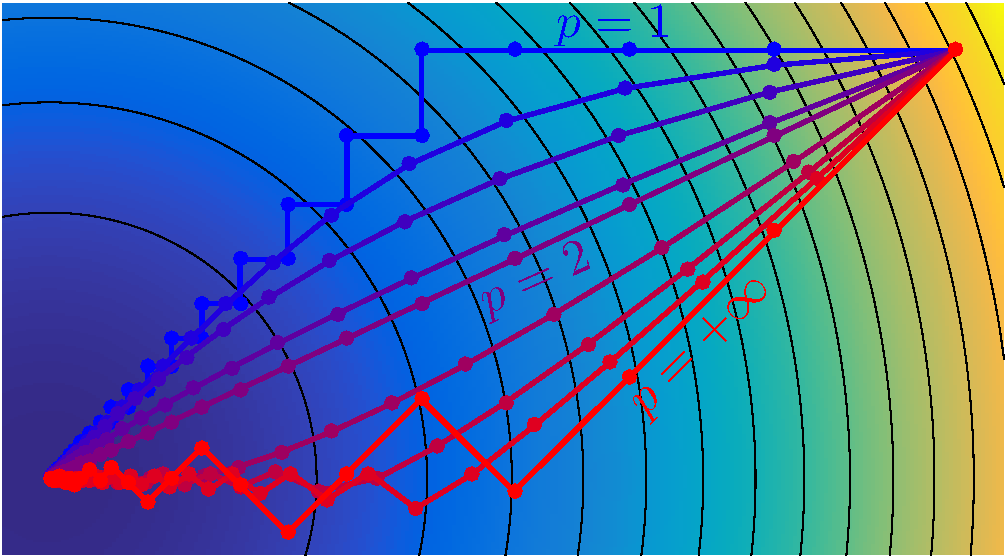
\includegraphics[width=.45\linewidth]{gradflow-metric/explicit}&
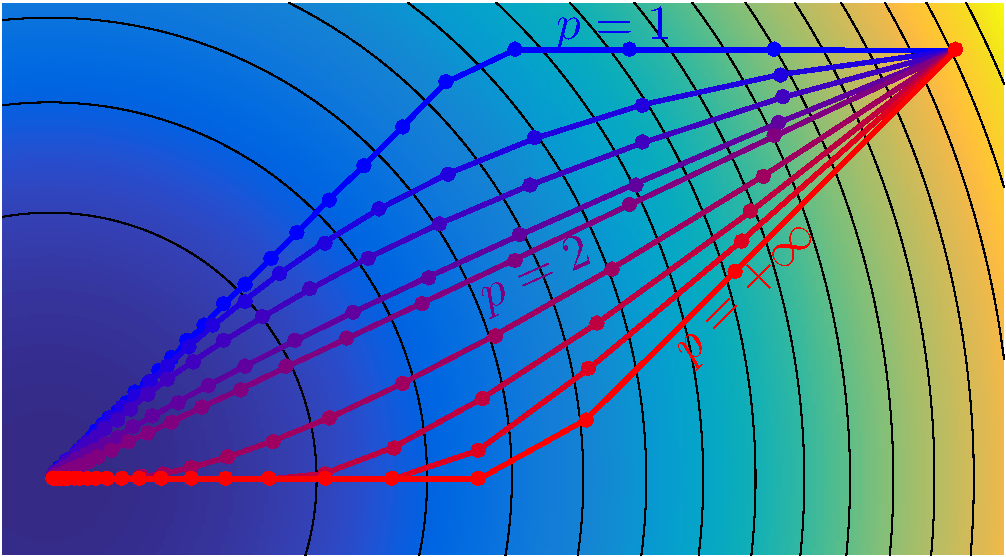
\includegraphics[width=.45\linewidth]{gradflow-metric/implicit}\\
Explicit & Implicit
\end{tabular}
\caption{\label{fig-gradflow-metric}
Comparison of explicit and implicit gradient flow to minimize the function $f(x) = \norm{x}^2$ on $\Xx=\RR^2$ for the distances $d(x,y)=\norm{x-y}_p$ for several values of $p$. 
}
\end{figure}


%%
\begin{rem1}{Lagrangian discretization using particles systems}\label{rem-lagr-discretization}
The finite-dimensional problem in~\eqref{eq-grad-flow-discr} can be interpreted as the Eulerian discretization of a flow over the space of measures~\eqref{eq-grad-flow-stepping-cont}.
%
An alternative way to discretize the problem, using the so-called Lagrangian method using particles systems, is to parameterize instead the solution as a (discrete) empirical measure moving with time, where the locations of that measure (and not its weights) become the variables of interest. In practice, one can consider a dynamic point cloud of particles $\al_t = \frac{1}{n}\sum_{i=1}^n \de_{x_i(t)}$ indexed with time.
%
The initial problem~\eqref{eq-grad-flow-discr} is then replaced by a set of $n$ coupled ODE prescribing the dynamic of the points $X(t)=(x_i(t))_i \in \X^n$. 
%
If the energy $F$ is finite for discrete measures, then one can simply define $\Ff(X)=F( \frac{1}{n}\sum_{i=1}^n \de_{x_i} )$. Typical examples are linear functions $F(\al) = \int_\X V(x) \d\al(x)$ and quadratic interactions $F(\al) = \int_{\X^2} W(x,y) \d\al(x)\d\al(y)$, in which case one can use respectively 
\eq{
	\Ff(X) = \frac{1}{n} \sum_i V(x_i) \qandq \Ff(X) = \frac{1}{n^2} \sum_{i,j} W(x_i,x_j). 
}
%
For functions such as generalized entropy, which are only finite for measures having densities, one should apply a density estimator to convert the point cloud into a density, which allows us to also define function $\Ff(x)$ consistent with $F$ as $n \rightarrow +\infty$. A typical example is for the entropy $F(\mu) = \H(\al)$ defined in~\eqref{eq-entropy-cont}, for which a consistent estimator (up to a constant term) can be obtained by summing the logarithms of the distances to nearest neighbors
\eql{\label{eq-entropy-discretized}
	\Ff(X) = \frac{1}{n}\sum_{i} \log( d_X(x_i) )
	\qwhereq d_X(x) = \umin{x' \in X, x' \neq x} \norm{x-x'};
}
see~\citet{beirlant1997nonparametric} for a review of nonparametric entropy estimators.
%
For small enough step sizes $\tau$, assuming $\X=\RR^\dim$, the Wasserstein distance $\Wass_2$ matches the Euclidean distance on the points, \ie if $|t-t'|$ is small enough, $\Ww_2(\al_t,\al_{t'})=\norm{X(t)-X(t')}$. The gradient flow is thus equivalent to the Euclidean flow on positions $X'(t) = -\nabla \Ff(X(t))$, which is discretized for times $t_k=\tau k$ similarly to~\eqref{eq-explicit-euclidean} using explicit Euler steps
\eq{
	\itt{X} \eqdef \it{X} - \tau \nabla \Ff(\it{X}).
} 
%
Figure~\ref{fig-flow-lagr} shows an example of such a discretized explicit evolution for a linear plus entropy functional, resulting in a discretized version of a Fokker--Planck equation.   
%
Note that for this particular case of linear Fokker--Planck equation, it is possible also to resort to stochastic PDEs methods, and it can be approximated numerically by evolving a single random particle with a Gaussian drift. The convergence of these schemes (so-called Langevin Monte Carlo) to the stationary distribution can in turn be quantified in terms of Wasserstein distance; see, for instance,~\citep{dalalyan2017user}. \todoK{Detailed this much more.}
%
If the function $\Ff$ is not smooth, one should discretize similarly to~\eqref{eq-implicit-euclidean} using implicit Euler steps, \ie consider 
\eq{
	\itt{X} \eqdef \Prox_{\tau \Ff}^{\norm{\cdot}}(\it{X}) \eqdef \uargmin{Z \in \X^n} \frac{1}{2}\norm{Z-\it{X}}^2 + \tau \Ff(Z).
}
%
In the simplest case of a linear function $F(\al) = \int_X V(x) \d\al(x)$, the flow operates independently over each particule $x_i(t)$ and corresponds to a usual Euclidean flow for the function $V$, $x_i'(t)=-\nabla V(x_i(t))$ (and is an advection PDEs of the density along the integral curves of the flow).
\end{rem1}

\newcommand{\FigLagrFlow}[1]{\includegraphics[width=.19\linewidth]{lagrangian-flows/lagrange-flow-#1}}


\begin{figure}[h!]
\centering
\begin{tabular}{@{}c@{}c@{}c@{}c@{}c@{}}
\FigLagrFlow{1} & 
\FigLagrFlow{3} & 
\FigLagrFlow{5} & 
\FigLagrFlow{7} & 
\FigLagrFlow{10} \\
$t=0$ & $t=0.2$  & $t=0.4$ & $t=0.6$ & $t=0.8$
\end{tabular}
\caption{\label{fig-flow-lagr}
Example of gradient flow evolutions using a Lagrangian discretization, for the function $F(\al) = \int V \d\al - H(\al)$, for $V(x)=\norm{x}^2$.
%
The entropy is discretized using~\eqref{eq-entropy-discretized}.
% 
The limiting stationary distribution is a Gaussian. 
}
\end{figure}


%%%%%%%%%%%%%%%%%%
\begin{rem2}{Geodesic convexity}
An important concept related to gradient flows is the convexity of the functional $F$ with respect to the Wasserstein-2 geometry, \ie the convexity of $F$ along Wasserstein geodesics (\ie displacement interpolations as shown in Remark~\ref{rem-displacement}). The Wasserstein gradient flow (with a continuous time) for such a function exists, is unique, and is the limit of the discrete stepping~\eqref{eq-grad-flow-stepping-cont} as $\tau \rightarrow 0$. It converges to a fixed stationary distribution as $t \rightarrow +\infty$.    
%
The entropy is a typical example of geodesically convex function, and so are linear functions of the form $F(\al) = \int_\X V(x) \d\al(x)$ and quadratic interaction functions $F(\al) = \int_{\X \times \X} W(x,y) \d\al(x) \d\al(y)$ for convex functions $V : \X \rightarrow \RR$, $W : \X \times \X \rightarrow \RR$. 
%
Note that while linear functions are convex in the classical sense, quadratic interaction functions might fail to be.
%
A typical example is $W(x,y)=\norm{x-y}^2$, which is a negative semi-definite kernel (see Definition~\ref{def-negativedefinitekernel}) and thus corresponds to $F(\al)$ being a concave function in the usual sense (while it is geodesically convex).  
%
An important result of~\citet{mccann1997convexity} is that generalized ``entropy'' functions of the form $F(\al) = \int_{\RR^\dim} \phi(\density{\al}(x)) \d x$ on $\X=\RR^\dim$ are geodesically convex if $\phi$ is convex, with $\phi(0)=0$, $\phi(t)/t \rightarrow +\infty$ as $t \rightarrow +\infty$ and such that  $s \mapsto s^{\dim} \phi(s^{-\dim})$ is convex decaying.
\end{rem2}
%%%%%%%%%%%%%%%%%%%

There is important literature on the numerical resolution of the resulting discretized flow, and we give only a few representative publications. For 1-D problems, very precise solvers have been developed because OT is a quadratic functional in the inverse cumulative function (see Remark~\ref{rem-1d-ot-generic}):~\citet{kinderlehrer1999approximation,blanchet2008convergence,agueh2013one,Matthes1D,blanchet2012optimal}. In higher dimensions, it can be tackled using finite elements and finite volume schemes:~\citet{CarrilloFiniteVolume,burger2010mixed}. Alternative solvers are obtained using Lagrangian schemes (\ie particles systems):~\citet{carrillo2009numerical,JDB-JKO,Westdickenberg2010}.
%
Another direction is to look for discrete flows (typically on discrete grids or graphs) which maintain some properties of their continuous counterparts; see~\citet{MielkeCVPDE,ErbarDCDS,ChowHuangLiZhou2012,Maas2011}.


An approximate approach to solve the Eulerian discretized problem~\eqref{eq-explicit-euclidean} relying on entropic regularization was initially proposed in~\citet{2015-Peyre-siims}, refined in~\citet{2016-chizat-sinkhorn} and theoretically analyzed in~\citet{2017-carlier-SIMA}.
%
With an entropic regularization, Problem~\eqref{eq-grad-flow-discr} has the form~\eqref{eq-generalized-ot-regul} when setting $G = \iota_{\it{\a}}$ and replacing $F$ by $\tau F$. One can thus use the iterations~\eqref{eq-gen-sinkh} to approximate $\itt{\a}$ as proposed initially in~\citet{2015-Peyre-siims}. The convergence of this scheme as $\epsilon \rightarrow 0$ is proved in~\citet{2017-carlier-SIMA}.
%
Figure~\ref{fig-jko} shows an example of evolution computed with this method.
%
An interesting application of gradient flows to machine learning is to learn the underlying function $F$ that best models some dynamical model of density. This learning can be achieved by solving a smooth nonconvex optimization using entropic regularized transport and automatic differentiation (see Remark~\ref{rem-auto-diff}); see~\citet{hashimoto2016learning}. 

Analyzing the convergence of gradient flows discretized in both time and space is difficult in general. Due to the polyhedral nature of the linear program defining the distance, using too-small step sizes leads to a ``locking'' phenomena (the distribution is stuck and does not evolve, so that the step size should be not too small, as discussed in~\citep{maury201713}). We refer to~\citep{Matthes1D,matthes2017convergent} for a convergence analysis of a discretization method for gradient flows in one dimension. 


\begin{figure}[h!]
\centering
\begin{tabular}{@{}c@{\hspace{1mm}}c@{\hspace{1mm}}c@{\hspace{1mm}}c@{\hspace{1mm}}c@{}}
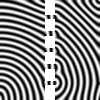
\includegraphics[width=.19\linewidth]{jko/congestion/holes-potential}&
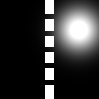
\includegraphics[width=.19\linewidth]{jko/congestion/holes-kappa10-1}&
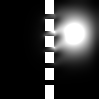
\includegraphics[width=.19\linewidth]{jko/congestion/holes-kappa10-2}&
% 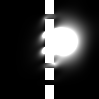
\includegraphics[width=.19\linewidth]{jko/congestion/holes-kappa10-5}&
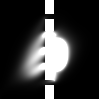
\includegraphics[width=.19\linewidth]{jko/congestion/holes-kappa10-10}&
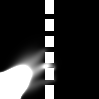
\includegraphics[width=.19\linewidth]{jko/congestion/holes-kappa10-20}\\
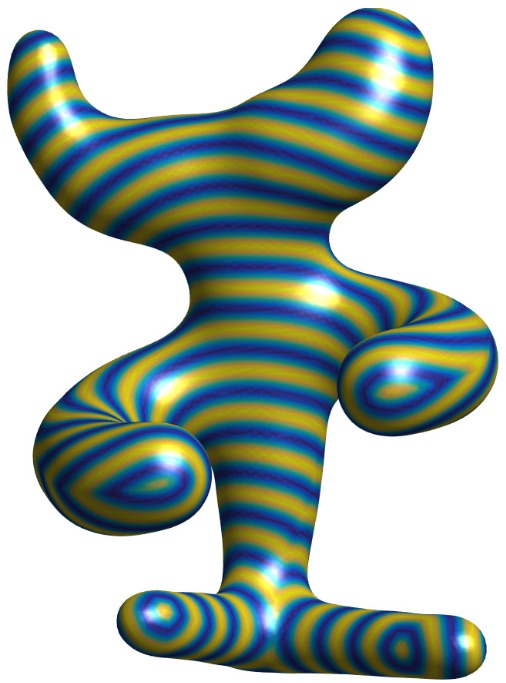
\includegraphics[width=.19\linewidth]{jko/surfaces/cosw}&
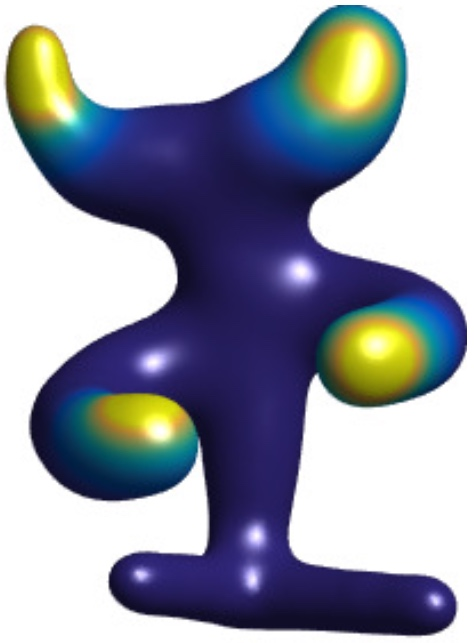
\includegraphics[width=.19\linewidth]{jko/surfaces/evol-1}&
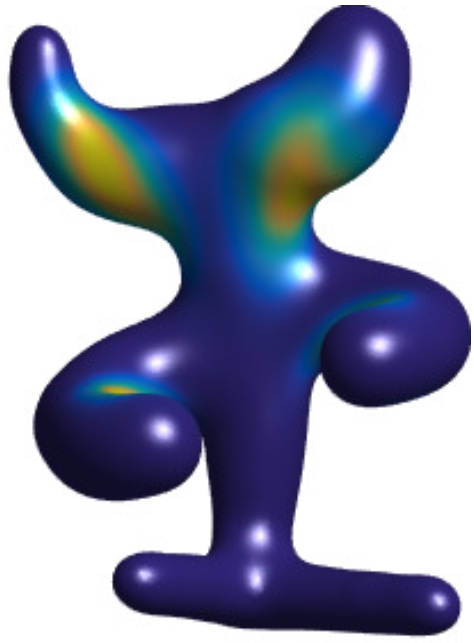
\includegraphics[width=.19\linewidth]{jko/surfaces/evol-2}&
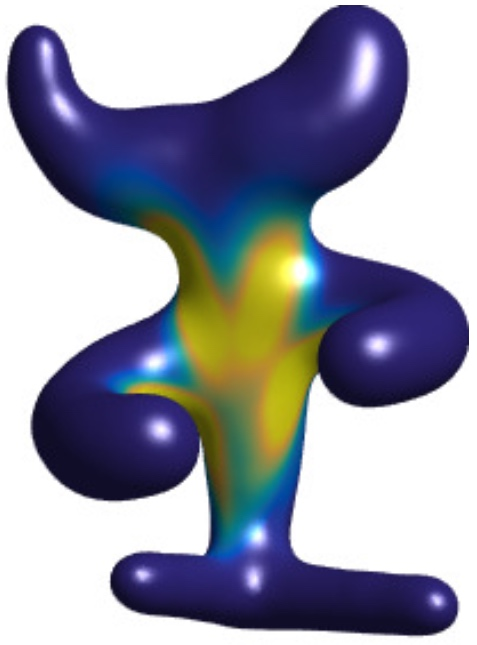
\includegraphics[width=.19\linewidth]{jko/surfaces/evol-3}&
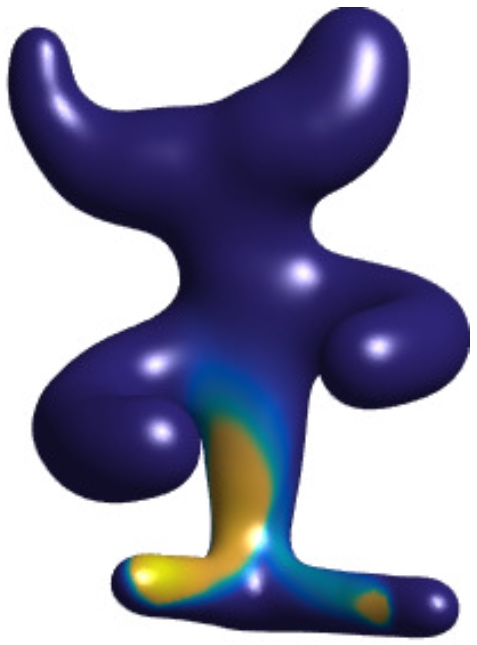
\includegraphics[width=.19\linewidth]{jko/surfaces/evol-4}\\
$\cos(w)$ & $t=0$ & $t=5$ & $t=10$ & $t=20$
\end{tabular}
\caption{\label{fig-jko}
Examples of gradient flows evolutions, with drift $V$ and congestion terms (from~\citet{2015-Peyre-siims}), so that $F(\al) = \int_\X V(x) \d \al(x) + \iota_{\leq \kappa}(\density{\al})$.
}
\end{figure}



It is also possible to compute gradient flows for unbalanced optimal transport distances as detailed in~\S\ref{sec-unbalanced}. This results in evolutions allowing mass creation or destruction, which is crucial to model many physical, biological or chemical phenomena. % Figure~\ref{fig-ot-grad-flows} shows 
An example of unbalanced gradient flow is the celebrated Hele-Shaw model for cell growth~\citep{PerthameTumor}, which is studied theoretically in~\citep{gallouet2017jko,marino2017tumor}. Such an unbalanced gradient flow also can be approximated using the generalized Sinkhorn algorithm~\citep{2016-chizat-sinkhorn}.


%\begin{figure}[h!]
%\centering
%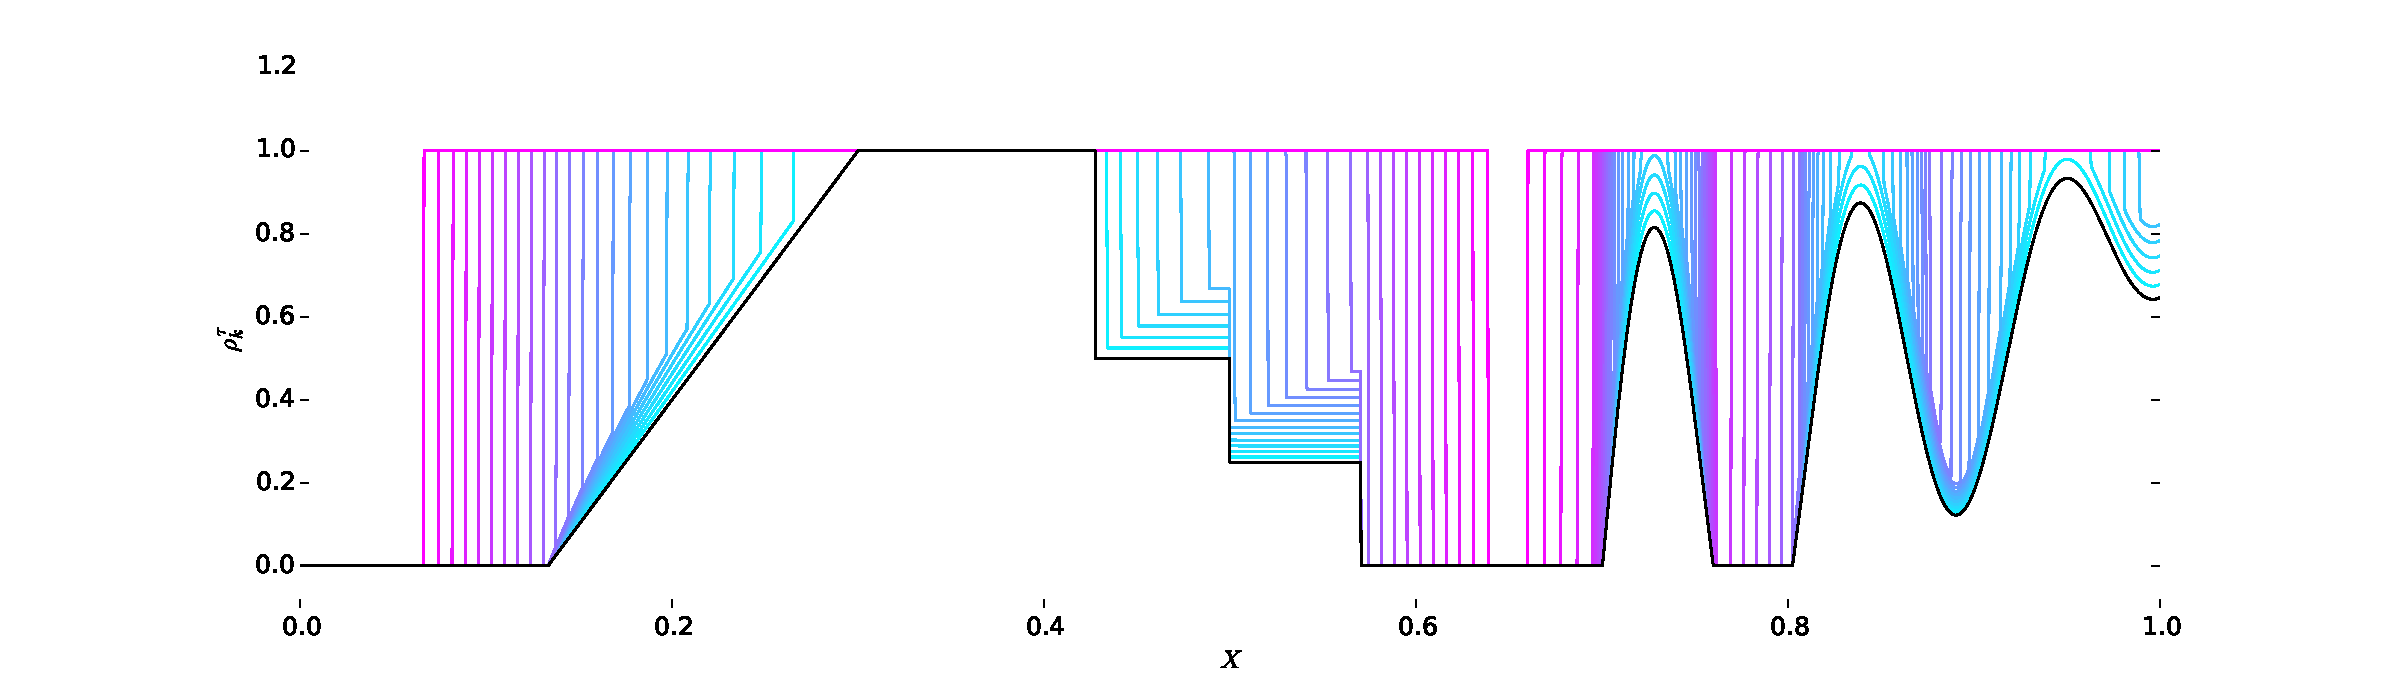
\includegraphics[width=.8\linewidth]{jko/heleshaw_profile}
%\caption{\label{fig-ot-grad-flows}
%Unbalanced OT gradient flow to solve the Hele-Shaw equation (from~\citep{2016-chizat-sinkhorn}). \todoK{detail the functional involved}
%}
%\end{figure}


%%%%%%%%%%%%%%%%%%%%%%%%%%%%%%%%%%%%%
%%%%%%%%%%%%%%%%%%%%%%%%%%%%%%%%%%%%%
%%%%%%%%%%%%%%%%%%%%%%%%%%%%%%%%%%%%%
%%%%%%%%%%%%%%%%%%%%%%%%%%%%%%%%%%%%%
\section{Minimum Kantorovich Estimators}
\label{sec-mke}

Given some discrete samples $(x_i)_{i=1}^n \subset \Xx$ from some unknown distribution, the goal is to fit a parametric model $\th \mapsto \al_\th \in \Mm(\Xx)$ to the observed empirical input measure $\be$
\eql{\label{eq-density-fitting}
	\umin{\th \in \Theta} \Ll(\al_\th,\be)
	\qwhereq
	\be = \frac{1}{n} \sum_i \de_{x_i}, 
}
where $\Ll$ is some ``loss'' function between a discrete and a ``continuous'' (arbitrary) distribution (see Figure~\ref{fig-density-fitting}). 

In the case where $\al_\th$ as a density $\density{\th} \eqdef \density{\al_\th}$ with respect to the Lebesgue measure (or any other fixed reference measure), the maximum likelihood estimator (MLE) is obtained by solving
\eq{
	\umin{\th} \Ll_{\text{MLE}}(\al_\th,\be) \eqdef -\sum_i \log(\density{\th}(x_i)). 
}
This corresponds to using an empirical counterpart of a Kullback--Leibler loss since, assuming the $x_i$ are i.i.d. samples of some $\bar\be$, then 
\eq{
	\Ll_{\text{MLE}}(\al,\be) \overset{n \rightarrow +\infty}{\longrightarrow} \KL(\al|\bar\be).
}

\begin{figure}[h!]
\centering
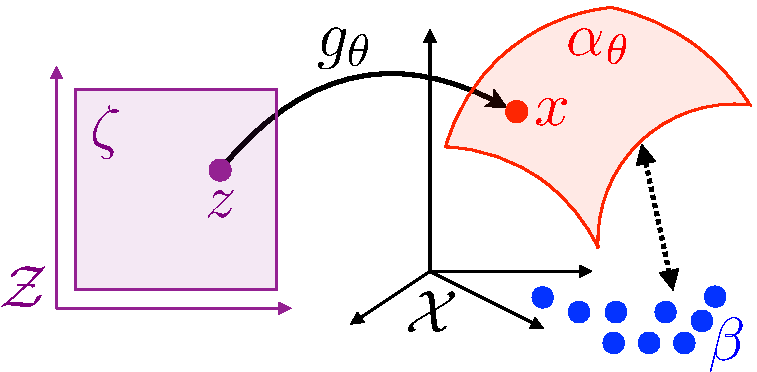
\includegraphics[width=.4\linewidth]{density-fitting/schematic-fitting}
\caption{\label{fig-density-fitting}
Schematic display of the density fitting problem~\ref{eq-density-fitting}.
}
\end{figure}


\newcommand{\fPF}{h}

This MLE approach is known to lead to optimal estimation procedures in many cases (see, for instance,~\citet{owen2001empirical}). However, it fails to work when estimating singular distributions, typically when the $\al_\th$ does not have a density (so that $\Ll_{\text{MLE}}(\al_\th,\be) = +\infty$) or when $(x_i)_i$ are samples from some singular $\bar\be$ (so that the $\al_\th$ should share the same support as $\be$ for $\KL(\al_\th|\bar\be)$ to be finite, but this support is usually unknown). Another issue is that in several cases of practical interest, the density $\density{\th}$ is inaccessible (or too hard to compute).

A typical setup where both problems (singular and unknown densities) occur is for so-called generative models, where the parametric measure is written as a push-forward of a fixed reference measure $\zeta \in \Mm(\Zz)$
\eq{
	\al_\th = \fPF_{\th,\sharp} \zeta \qwhereq \fPF_\th : \Zz \rightarrow \Xx,
}
where the push-forward operator is introduced in Definition~\ref{defn-pushfwd}. The space $\Zz$ is usually low-dimensional, so that the support of $\al_\th$ is localized along a low-dimensional ``manifold'' and the resulting density is highly singular (it does not have a density with respect to Lebesgue measure).
%
Furthermore, computing this density is usually intractable, while generating i.i.d. samples from $\al_\th$ is achieved by computing $x_i=\fPF_\th(z_i)$, where $(z_i)_i$ are i.i.d. samples from $\zeta$.

In order to cope with such a difficult scenario, one has to use weak metrics in place of the MLE functional $\Ll_{\text{MLE}}$, which needs to be written in dual form as 
\eql{\label{eq-dual-loss}
	\Ll(\al,\be) \eqdef 
	\umax{(\f,\g) \in \Cc(\X)^2} 
	\enscond{ \int_{\X} \f(x) \d\al(x) + \int_{\X} \g(x) \d\be(x) }{ (\f,\g) \in \Potentials}.
}
Dual norms shown in~\S\ref{sec-dual-norms} correspond to imposing 
\eq{
	\Potentials = \enscond{(\f,-\f)}{\f \in B}, 
}
while optimal transport~\eqref{eq-dual-generic} sets $\Potentials = \Potentials(\c)$ as defined in~\eqref{eq-dfn-pot-dual}. 

For a fixed $\th$, evaluating the energy to be minimized in~\eqref{eq-density-fitting} using such a loss function corresponds to solving a semidiscrete optimal transport, which is the focus of Chapter~\ref{c-algo-semidiscr}. Minimizing the energy with respect to $\th$ is much more involved and is typically highly nonconvex.

Denoting $\f_\th$ a solution to~\eqref{eq-dual-loss} when evaluating $\Ee(\th) = \Ll(\al_\th,\be)$, a subgradient is obtained using the formula
\eql{\label{eq-grad-wass-loss-dual}
	\nabla \Ee(\th) = \int_\Xx [\partial \fPF_\th(x)]^\top \nabla \f_\th(x) \d\al_\th(x), 
}
where $\partial \fPF_\th(x) \in \RR^{\text{dim}(\Theta) \times \dim}$ is the differential (with respect to $\th$) of $\th \in \RR^{\text{dim}(\Theta)} \mapsto \fPF_\th(x)$, while $\nabla \f_\th(x)$ is the gradient (with respect to $x$) of $\f_\th$. 
%
This formula is hard to use numerically, first because it requires first computing a continuous function $\f_\th$, which is a solution to a semi-discrete problem. As shown in~\S\ref{sec-entropy-ot-mmd}, for OT loss, this can be achieved using stochastic optimization, but this is hardly applicable in high dimension. Another option is to impose a parametric form for this potential, for instance expansion in an RKHS~(\citet{genevay2016stochastic}) or a deep-network approximation~(\citep{WassersteinGAN}). This, however, leads to important approximation errors that are not yet analyzed theoretically.
%
A last issue is that it is unstable numerically because it requires the computation of the gradient $\nabla \f_\th$ of the dual potential $\f_\th$.

For the OT loss, an alternative gradient formula is obtained when one rather computes a primal optimal coupling  for the following equivalent problem:
\eql{\label{eq-ot-couplings-fitting}
	\MK_\c(\al_\th,\be) = \umin{\ga \in \Mm(\Zz \times \Xx)} 
		\enscond{
			\int_{\Zz \times \Xx} c(\fPF_\th(z),x) \d\ga(z,x)
		}{
			\gamma \in \Couplings(\zeta,\be)
		}.
}
Note that in the semidiscrete case considered here, the objective to be minimized can be actually decomposed as 
\eql{\label{eq-ot-couplings-fitting-bis}
	\umin{(\ga_i)_{i=1}^n} \sum_{i=1}^n \int_\Zz c(\fPF_\th(z),x_i) \d \ga_i(z)
	\qwhereq
	\sum_{i=1}^n \ga_i = \zeta, \quad
	\int_\Zz \d\ga_i(z)  = \frac{1}{n}, 
}
where each $\ga_i \in \Mm_+^1(\Zz)$. 
%
Once an optimal $(\gamma_{\th,i})_i$ solving~\eqref{eq-ot-couplings-fitting-bis} is obtained, the gradient of $\Ee(\th)$ is computed as
\eq{
	\nabla \Ee(\th) = \sum_{i=1}^n \int_\Zz [\partial \fPF_\th(z)]^\top \nabla_1 c(\fPF_\th(z),x_i) \d \ga_i(z), 
}
where $\nabla_1 c(x,y) \in \RR^\dim$ is the gradient of $x \mapsto c(x,y)$. Note that as opposed to~\eqref{eq-grad-wass-loss-dual}, this formula does not involve computing the gradient of the potentials being solutions of the dual OT problem.

The class of estimators obtained using $\Ll=\MK_\c$, often called ``minimum Kantorovich estimators,'' was initially introduced in~\citep{bassetti2006minimum}; see also~\citep{CanasRosasco}. It has been used in the context of generative models by~\citep{CuturiBoltzman} to train restricted Boltzmann machines and in~\citep{bernton2017inference} in conjunction with approximate Bayesian computations.  Approximations of these computations using Deep Network are used to train deep generative models for both GAN~\citep{WassersteinGAN} and VAE~\citep{Bousquet2017}; see also~\citep{2017-Genevay-AutoDiff,2017-Genevay-gan-vae,salimans2018improving}. Note that the use of Sinkhorn divergences for parametric model fitting is used routinely for shape matching and registration, see~\citep{gold1998new,chui2000new,myronenko2010point,2017-feydy-miccai}.


\begin{rem1}{Metric learning and transfer learning}
	Let us insist on the fact that, for applications in machine learning, the success of OT-related methods very much depends on the choice of an adapted cost $c(x,y)$ which captures the geometry of the data. 
	%
	While it is possible to embed many kinds of data in Euclidean spaces (see, for instance,~\citep{mikolov2013efficient} for words embedding), in many cases, some sort of adaptation or optimization of the metric is needed. 
	% 
	Metric learning for supervised tasks is a classical problem (see, for instance,~\citep{MAL-019,weinberger2009distance}) and it has been extended to the learning of the ground metric $c(x,y)$ when some OT distance is used in a learning pipeline~\citep{CuturiGroundMetric2014} (see also~\citealt{ZenICPR14,WangECCV12OLD,huang2016supervised}).
	%
	Let us also mention the related inverse problem of learning the cost matrix from the observations of an optimal coupling $\P$, which can be regularized using a low-rank prior~\citep{dupuy2016estimating}.
	%	
	Related problems are transfer learning~\citep{pan2010survey} and domain adaptation~\citep{glorot2011domain}, where one wants to transfer some trained machine learning pipeline to adapt it to some new dataset. This problem can be modeled and solved using OT techniques; see~\citep{courty2017optimal,courty2017joint}.
\end{rem1}

